\documentclass{beamer}
\usepackage[portuguese]{babel}
\usepackage[utf8x]{inputenc}
\usepackage{hyperref}
\usepackage{natbib}
\usepackage{amsmath}
\usepackage{amsthm}
\usepackage{amsfonts}
\usepackage{graphicx}
\usepackage{lmodern}
\usepackage{listings}

\usetheme{Ilmenau}
\usecolortheme{rose}

\beamertemplatenavigationsymbolsempty

% Parametrizando o estilo da linguagem usando pacote Listings
\lstset{
	basicstyle=\small\ttfamily,
	extendedchars=true,
	showspaces=false,
	showstringspaces=false,
	numbers=left,
	frame=tb,
	numberstyle=\tiny,
	breaklines=true,
	breakautoindent=true,
	captionpos=b,
	xleftmargin=0pt,
	tabsize=4
}

\title{Otimização de imagens de microscópio de contraste de fase
  para quantificação de confluência}

\author[Alan Sabino]{Alan Utsuni Sabino\\ {\tiny alan.sabino@usp.br}}

\institute[]
{
	\inst{}
	SIN5014 - Fundamentos de Processamento Gráfico \\
  % Instituto do Câncer do Estado de São Paulo\\
  % Faculdade de Medicina\\
  Universidade de São Paulo
}

\date{\today}

\setbeamertemplate{headline}
{%
  \begin{beamercolorbox}{section in head/foot}
    \insertsectionnavigationhorizontal{\textwidth}{}{}
  \end{beamercolorbox}%
}

\defbeamertemplate*{footline}{myminiframes theme}
{%
  \begin{beamercolorbox}[colsep=1.5pt]{upper separation line foot}
  \end{beamercolorbox}
  \begin{beamercolorbox}[ht=2.5ex,dp=1.125ex,%
    leftskip=.3cm,rightskip=.3cm plus1fil]{author in head/foot}%
    \leavevmode{\usebeamerfont{author in head/foot}\insertshortauthor}%
    \hfill%
    {\usebeamerfont{institute in head/foot}\usebeamercolor[fg]{institute in head/foot}\insertshortinstitute}%
  \end{beamercolorbox}%
  \begin{beamercolorbox}[ht=2.5ex,dp=1.125ex,%
    leftskip=.3cm,rightskip=.3cm plus1fil]{title in head/foot}%
    {\usebeamerfont{title in head/foot}\insertshorttitle\hfill \insertframenumber/\inserttotalframenumber}%<-here
  \end{beamercolorbox}%
  \begin{beamercolorbox}[colsep=1.5pt]{lower separation line foot}
  \end{beamercolorbox}
}

\makeatother

% ----------------------------------------------------------------------------------------
%	DOCUMENTO
% ----------------------------------------------------------------------------------------

\begin{document}

\label{Titulo}
{
  \begin{frame}[plain,noframenumbering]
    \titlepage
  \end{frame}
}

%\begin{frame}[allowframebreaks]{Tópicos}
%  \tableofcontents
%\end{frame}

\section{Objetivo}

\subsection{}
\begin{frame}{Objetivo}

  \begin{figure}
    \includegraphics[width=0.65\textwidth]{imgs/old_obj.png}\\
    \includegraphics[width=0.2\textwidth]{imgs/seta.png}\\
\includegraphics[width=0.65\textwidth]{imgs/new_obj.png}
    \end{figure}
\end{frame}

\begin{frame}{Contexto}

   \begin{columns}
    \column{0.45\textwidth}
    \begin{figure}
      \includegraphics[width=1.1\textwidth]{imgs/pcm.png}\\
      \includegraphics[width=1.1\textwidth]{imgs/conflu.png}
    \end{figure}

    \column{0.55\textwidth}
    \begin{itemize}
    \item Confluência: momento em que a linhagem celular cobre toda a placa,
      formando um tapete de células
      \vfill
    \item Comportamento das células é influenciado pela confluência
      \vfill
    \item Na prática, medida subjetiva que afeta reprodutibilidade e/ou repetição
      de ensaio e/ou experimento
    %\item Algoritmos disponíveis podem não ser eficientes em alguns casos

    \end{itemize}
  \end{columns}
\end{frame}

\section{Metodologia}
\begin{frame}{Banco de imagens}

    \begin{figure}
      \includegraphics[width=1\textwidth]{imgs/banco.png}
    \end{figure}

\end{frame}

\begin{frame}{Conceitos e técnicas}
     \begin{itemize}
     \item Remoção de ruído (Filtro Mediana 3x3)
     \item Aumento de contraste (Equalização)
     \item Detecção de bordas
     \end{itemize}

     \vfill

     Técnicas foram utilizadas com diferentes parâmetros e com pipelines de execução
     distintos.

\end{frame}

\section{Resultados obtidos}
\begin{frame}{Exemplo de pipeline}
  \begin{figure}
      \includegraphics[width=0.33\textwidth]{imgs/fototif.png}
      \includegraphics[width=0.33\textwidth]{imgs/mediana.png}
      \includegraphics[width=0.33\textwidth]{imgs/contraste.png}
      \includegraphics[width=0.33\textwidth]{imgs/bordas.png}
    \end{figure}

  \end{frame}

  \section{Próximos passos}
  \begin{frame}{Avaliação com algoritmos}

    \begin{figure}
      \includegraphics[width=0.3\textwidth]{imgs/fiji.png}
      \includegraphics[width=0.35\textwidth]{imgs/bioed.jpeg}
    \end{figure}

    \vfill

    \begin{itemize}
    \item Ajustar e criar novos pipelines de processamento
    \item Executar pipelines com as aplicações já desenvolvidas
 \item Avaliar performance dos algoritmos (Tempo de execução)
    \end{itemize}

  \end{frame}

  \begin{frame}{Automatização e comparar performance}

    \begin{itemize}

    \item Integrar script com pipelines e programas
    \item Avaliar se houve aumento de acurácia
    \end{itemize}

    \begin{figure}
      \includegraphics[width=0.4\textwidth]{imgs/fototif.png}
      \includegraphics[width=0.4\textwidth]{imgs/manual.png}
    \end{figure}

  \end{frame}

%\subsection{Resultados preliminares}
%\begin{frame}{Modelo para  melanoma}
%  \begin{columns}
%    \column{0.45\textwidth}
%    \begin{figure}
%      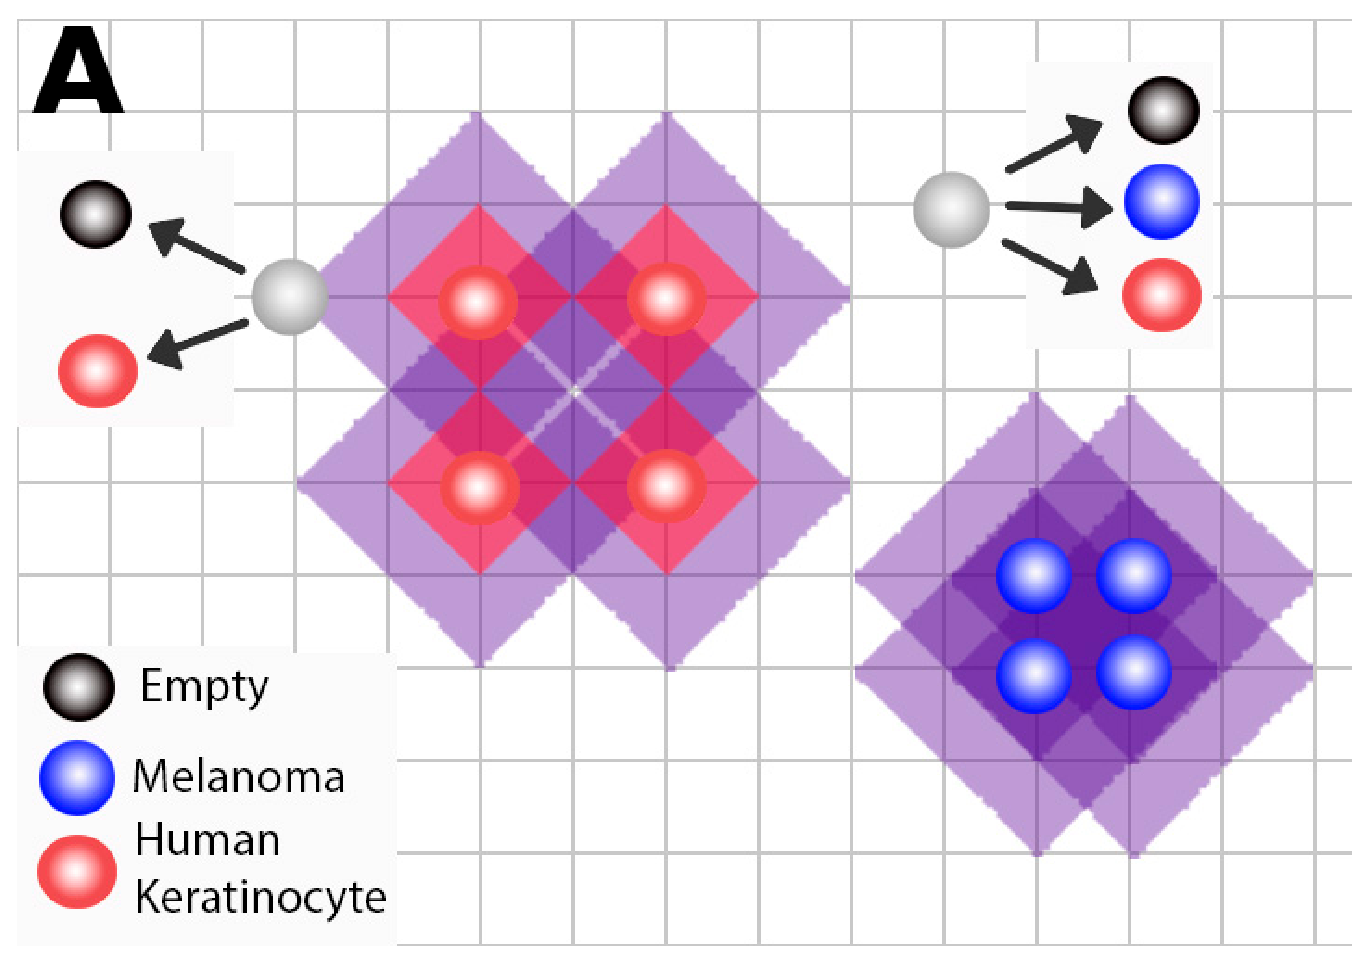
\includegraphics[width=1.22\textwidth]{imgs/gradeModelo.eps}
%    \end{figure}
%
%    \column{0.55\textwidth}
%    \begin{itemize}
%    \item Dinâmica do padrão espacial. A população de células
%      tumorais cresce até prevalecer todo o domínio.
%      \vfill
%    \item Borda preenchida com células normais. Diâmetros de
%      exclusão se mostram determinantes para a prevalência do tipo
%      celular no estado estacionário.
%      \vfill
%    \item Aleatoriedade intrínseca. Na ausência de um fator que
%      diferencie os tipos celulares será a estocasticidade do
%      sistema que indicará qual tipo celular irá prevalecer.
%    \end{itemize}
%  \end{columns}
%\end{frame}

%\begin{frame}{Modelo para  melanoma} % Segundo
%  \begin{columns}
%    \column{0.45\textwidth}
%    \begin{figure}
%      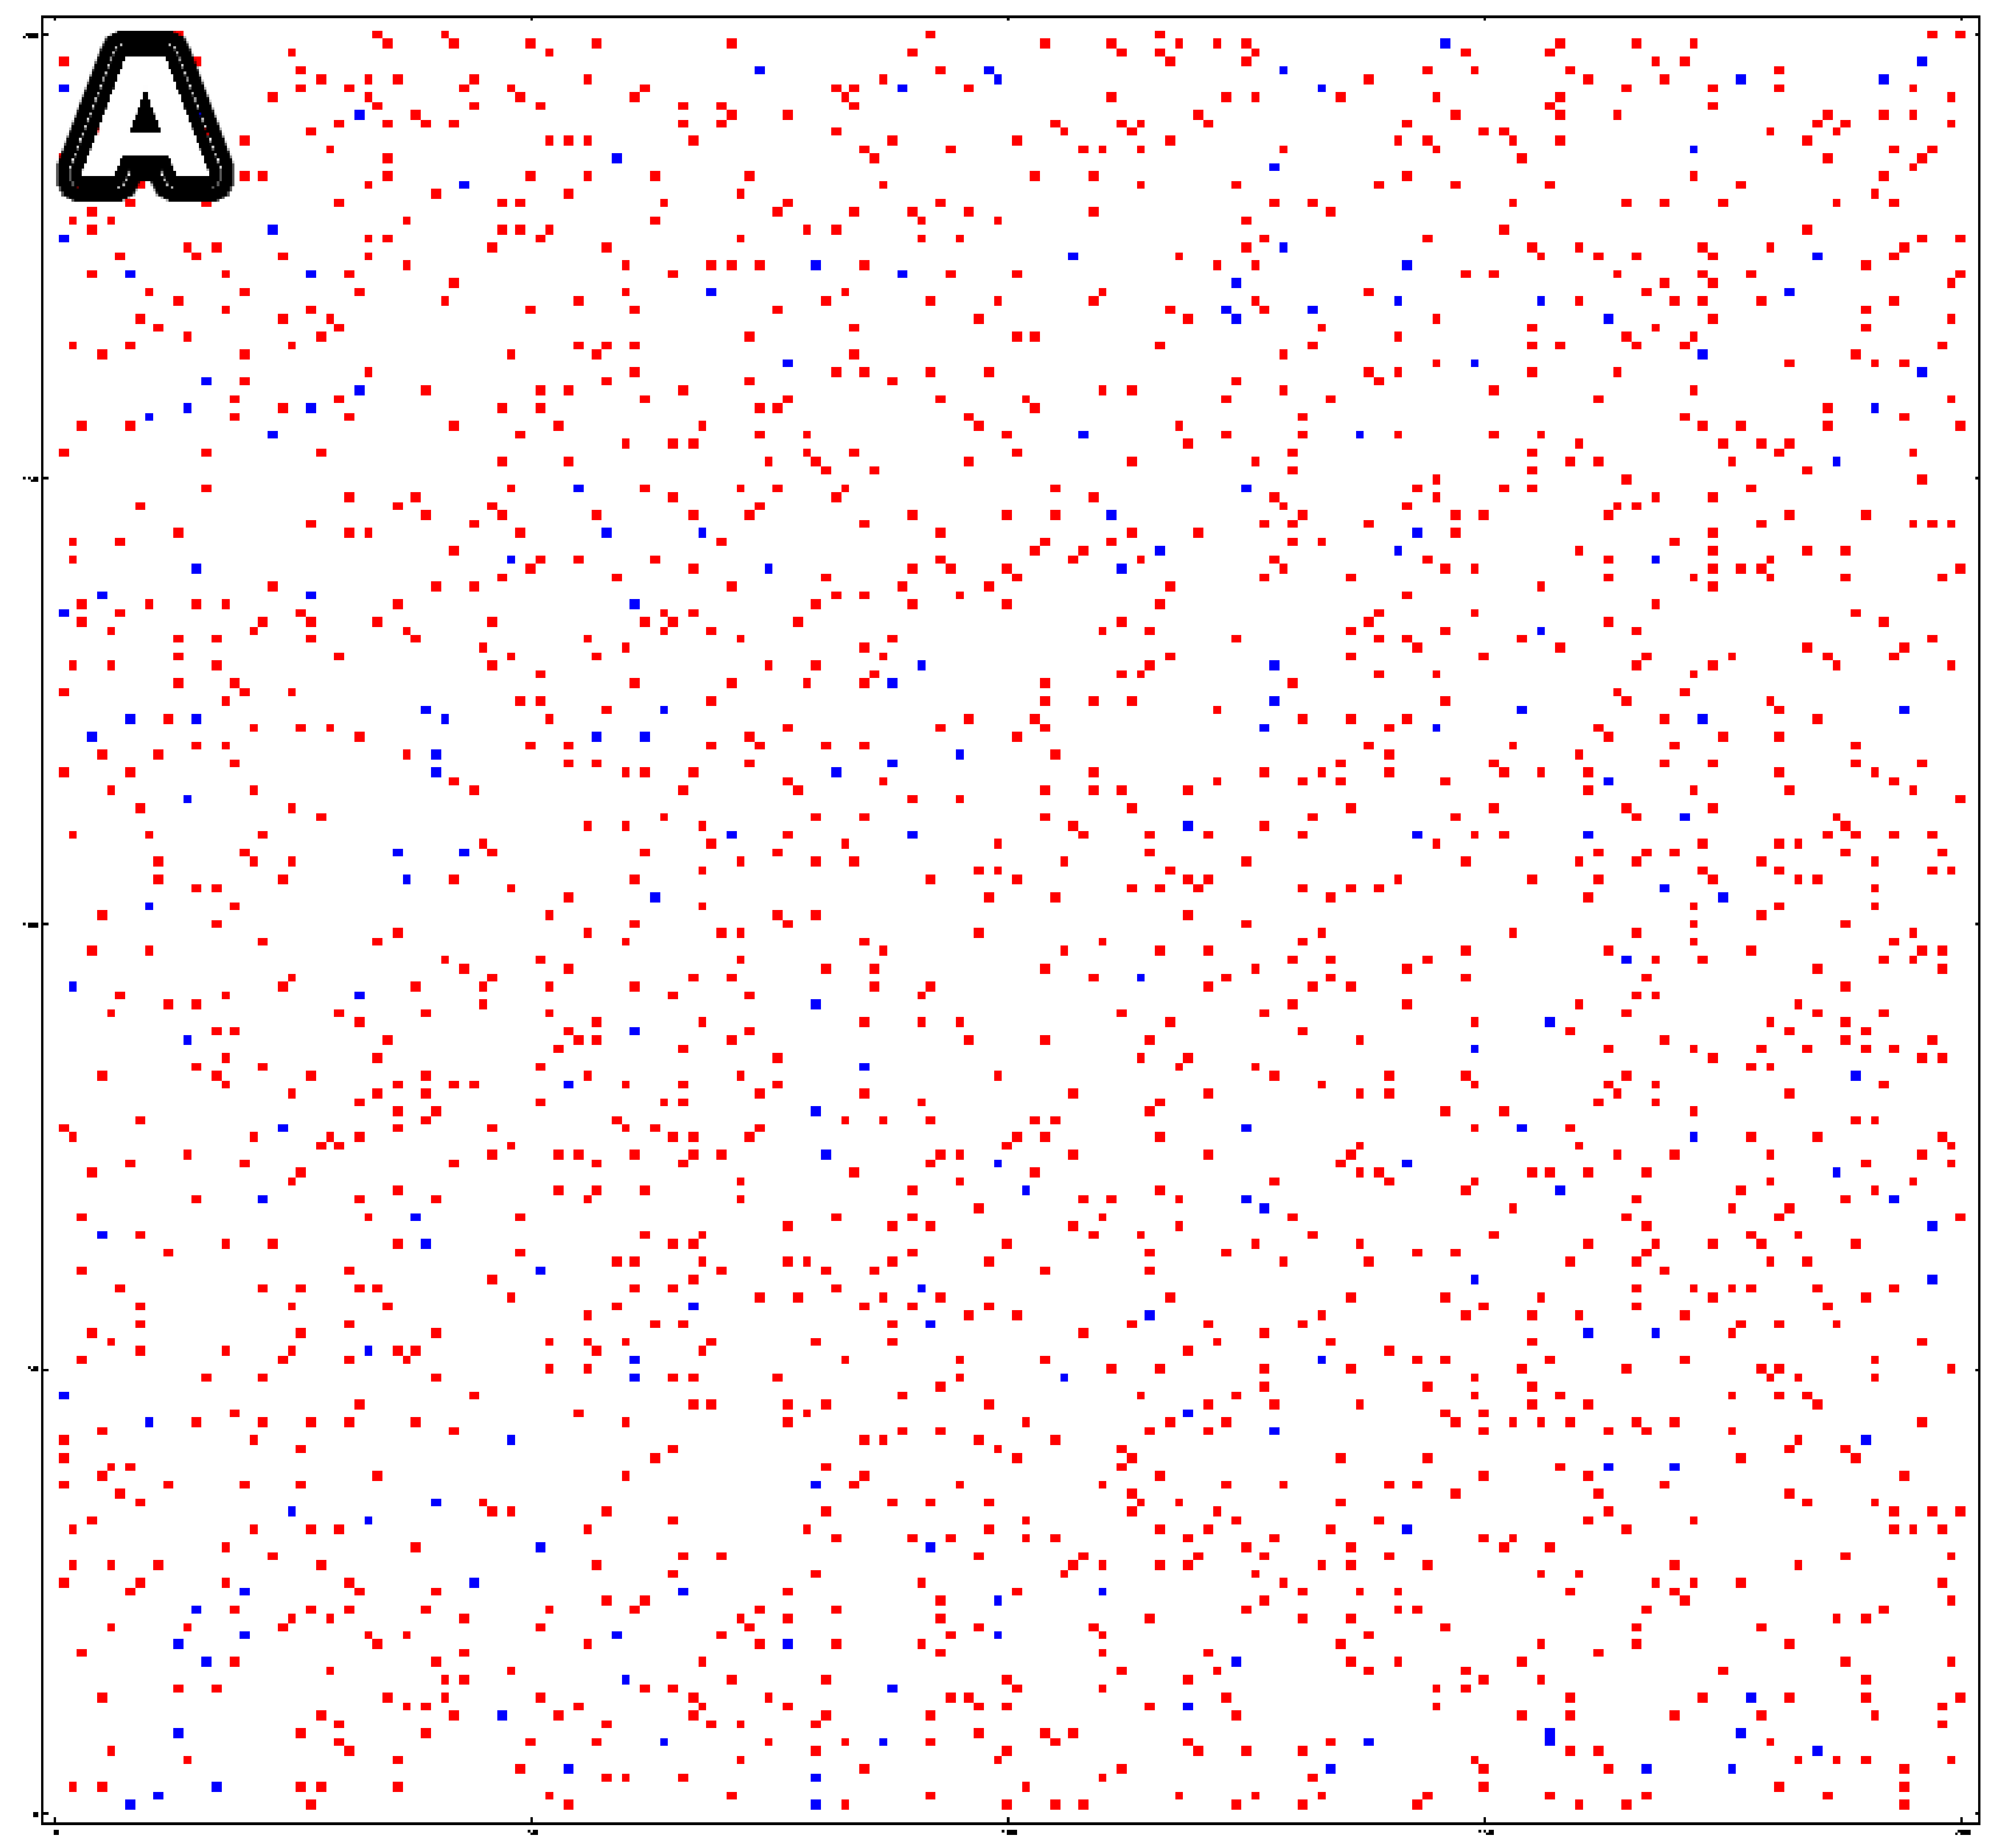
\includegraphics[width=0.25\textwidth]{imgs/0_021_heat1.eps}
%      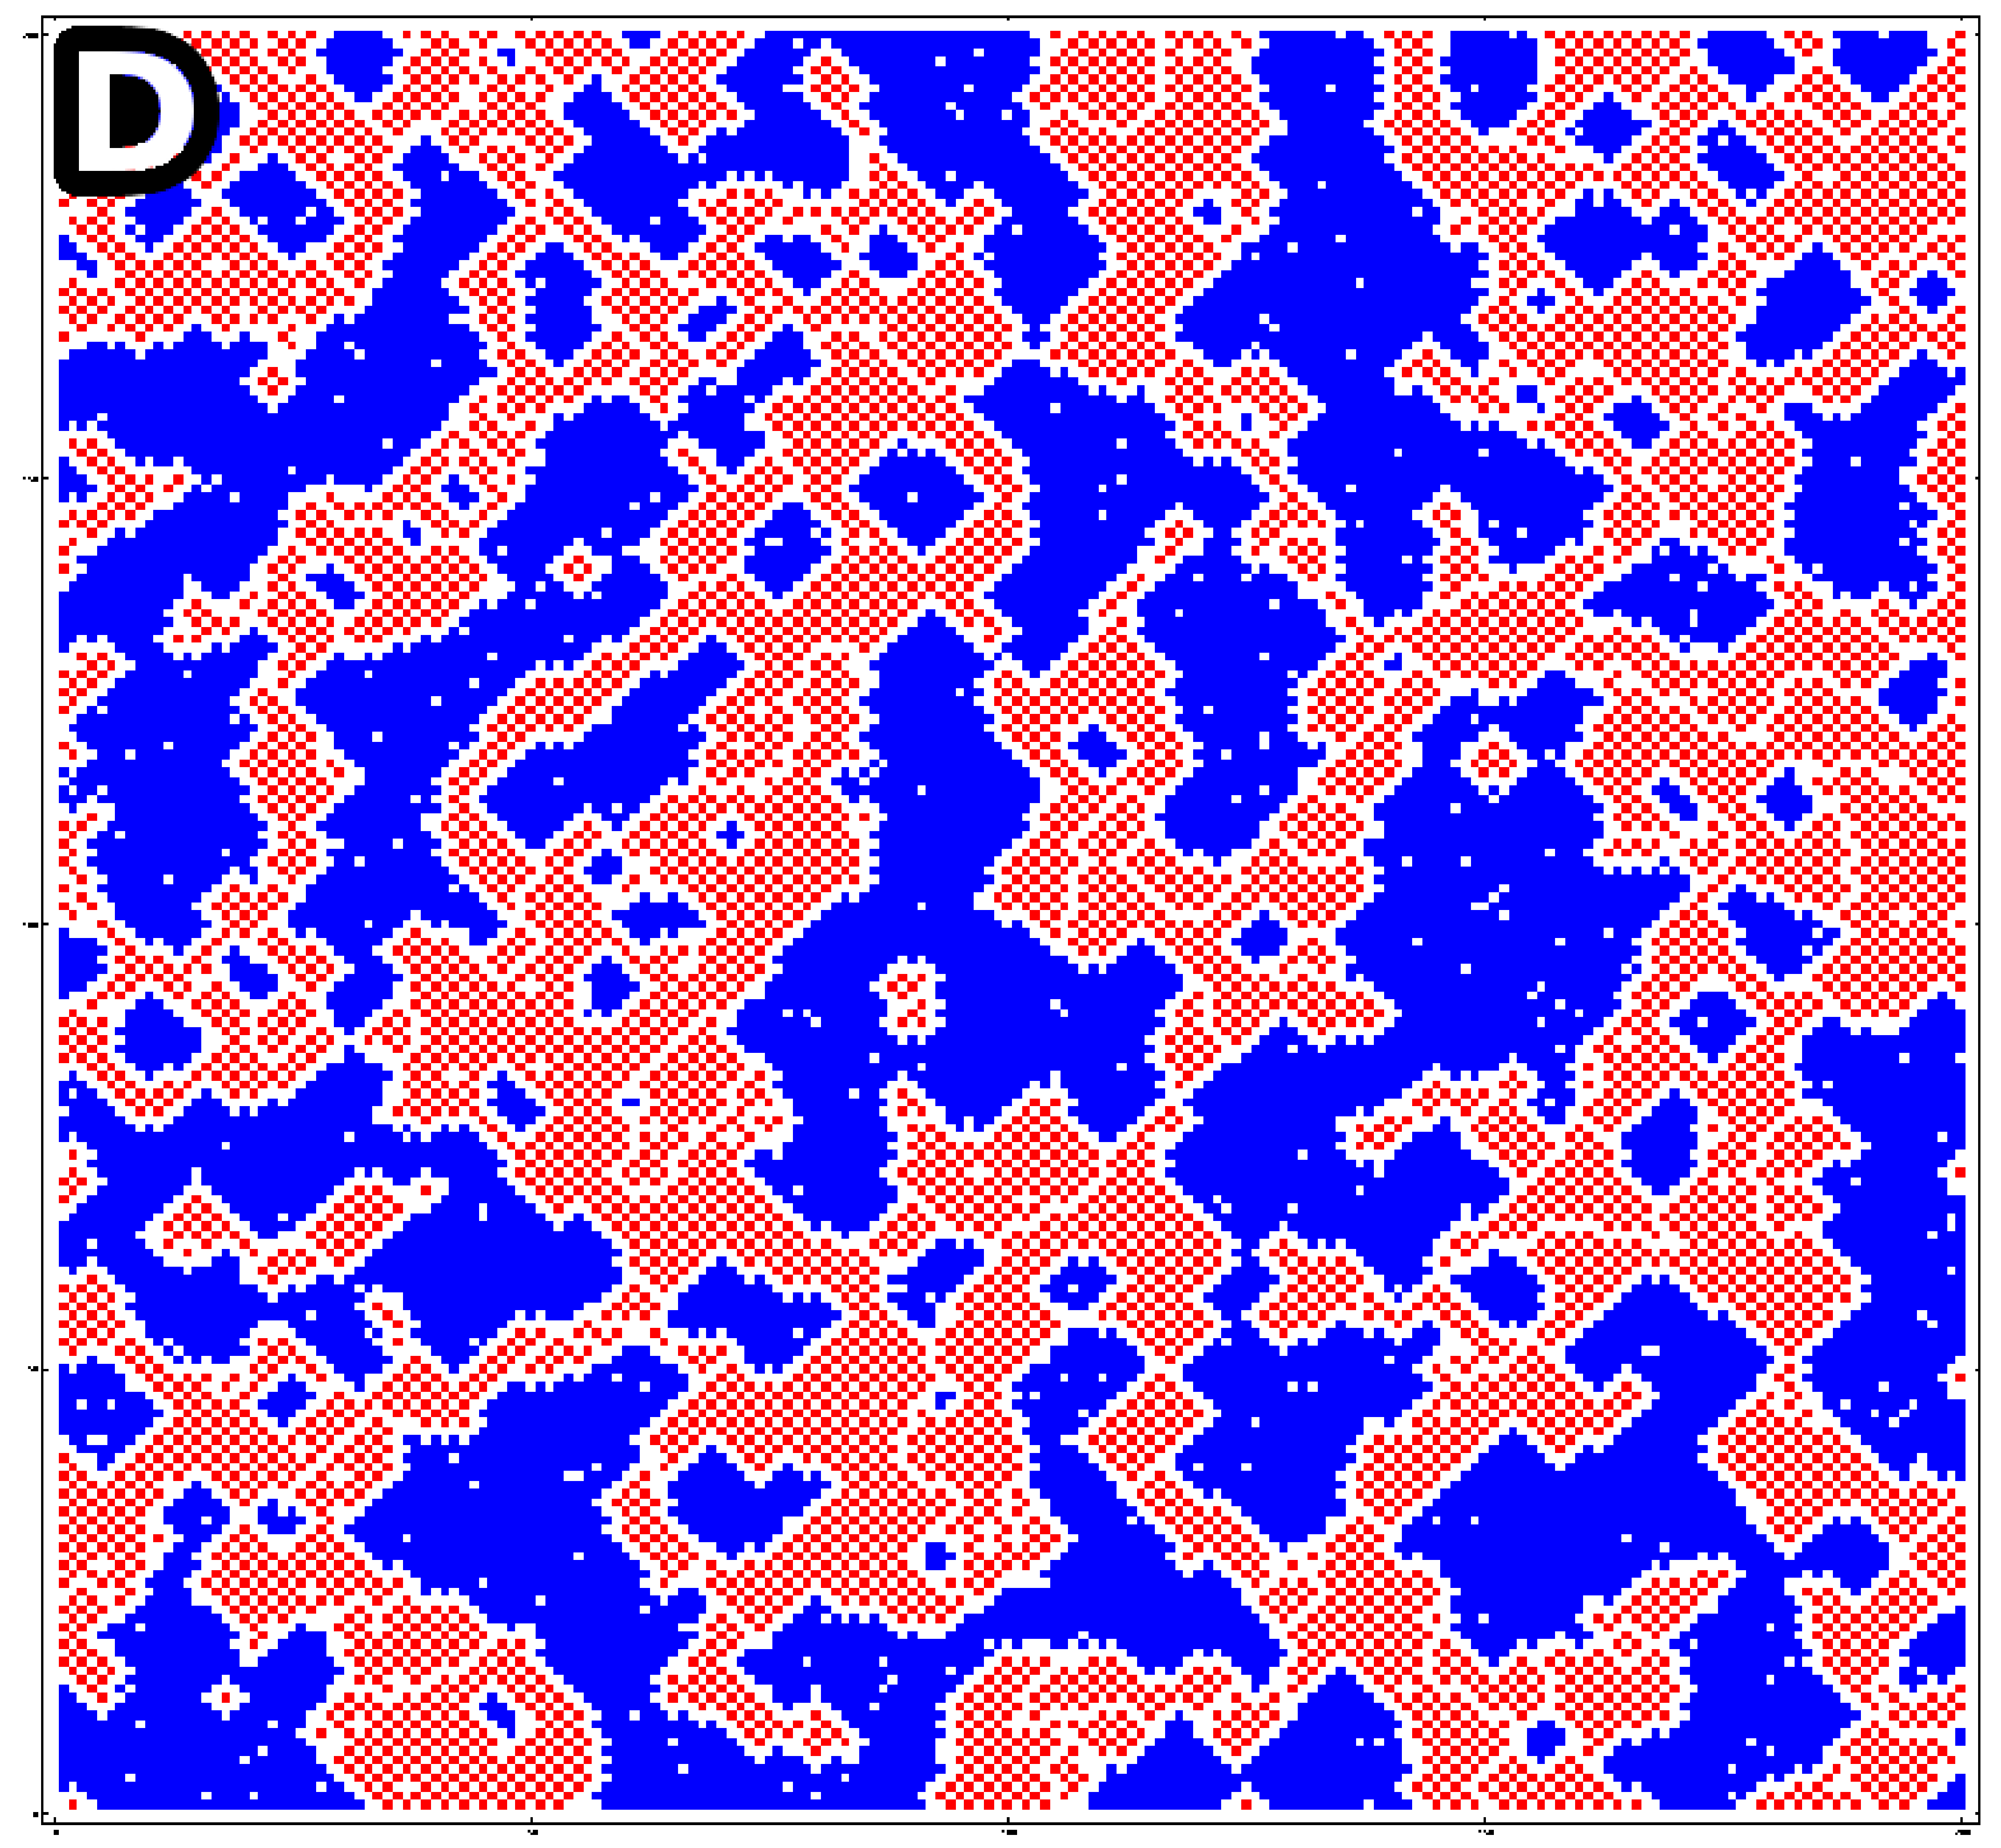
\includegraphics[width=0.25\textwidth]{imgs/0_021_heat64.eps}
%      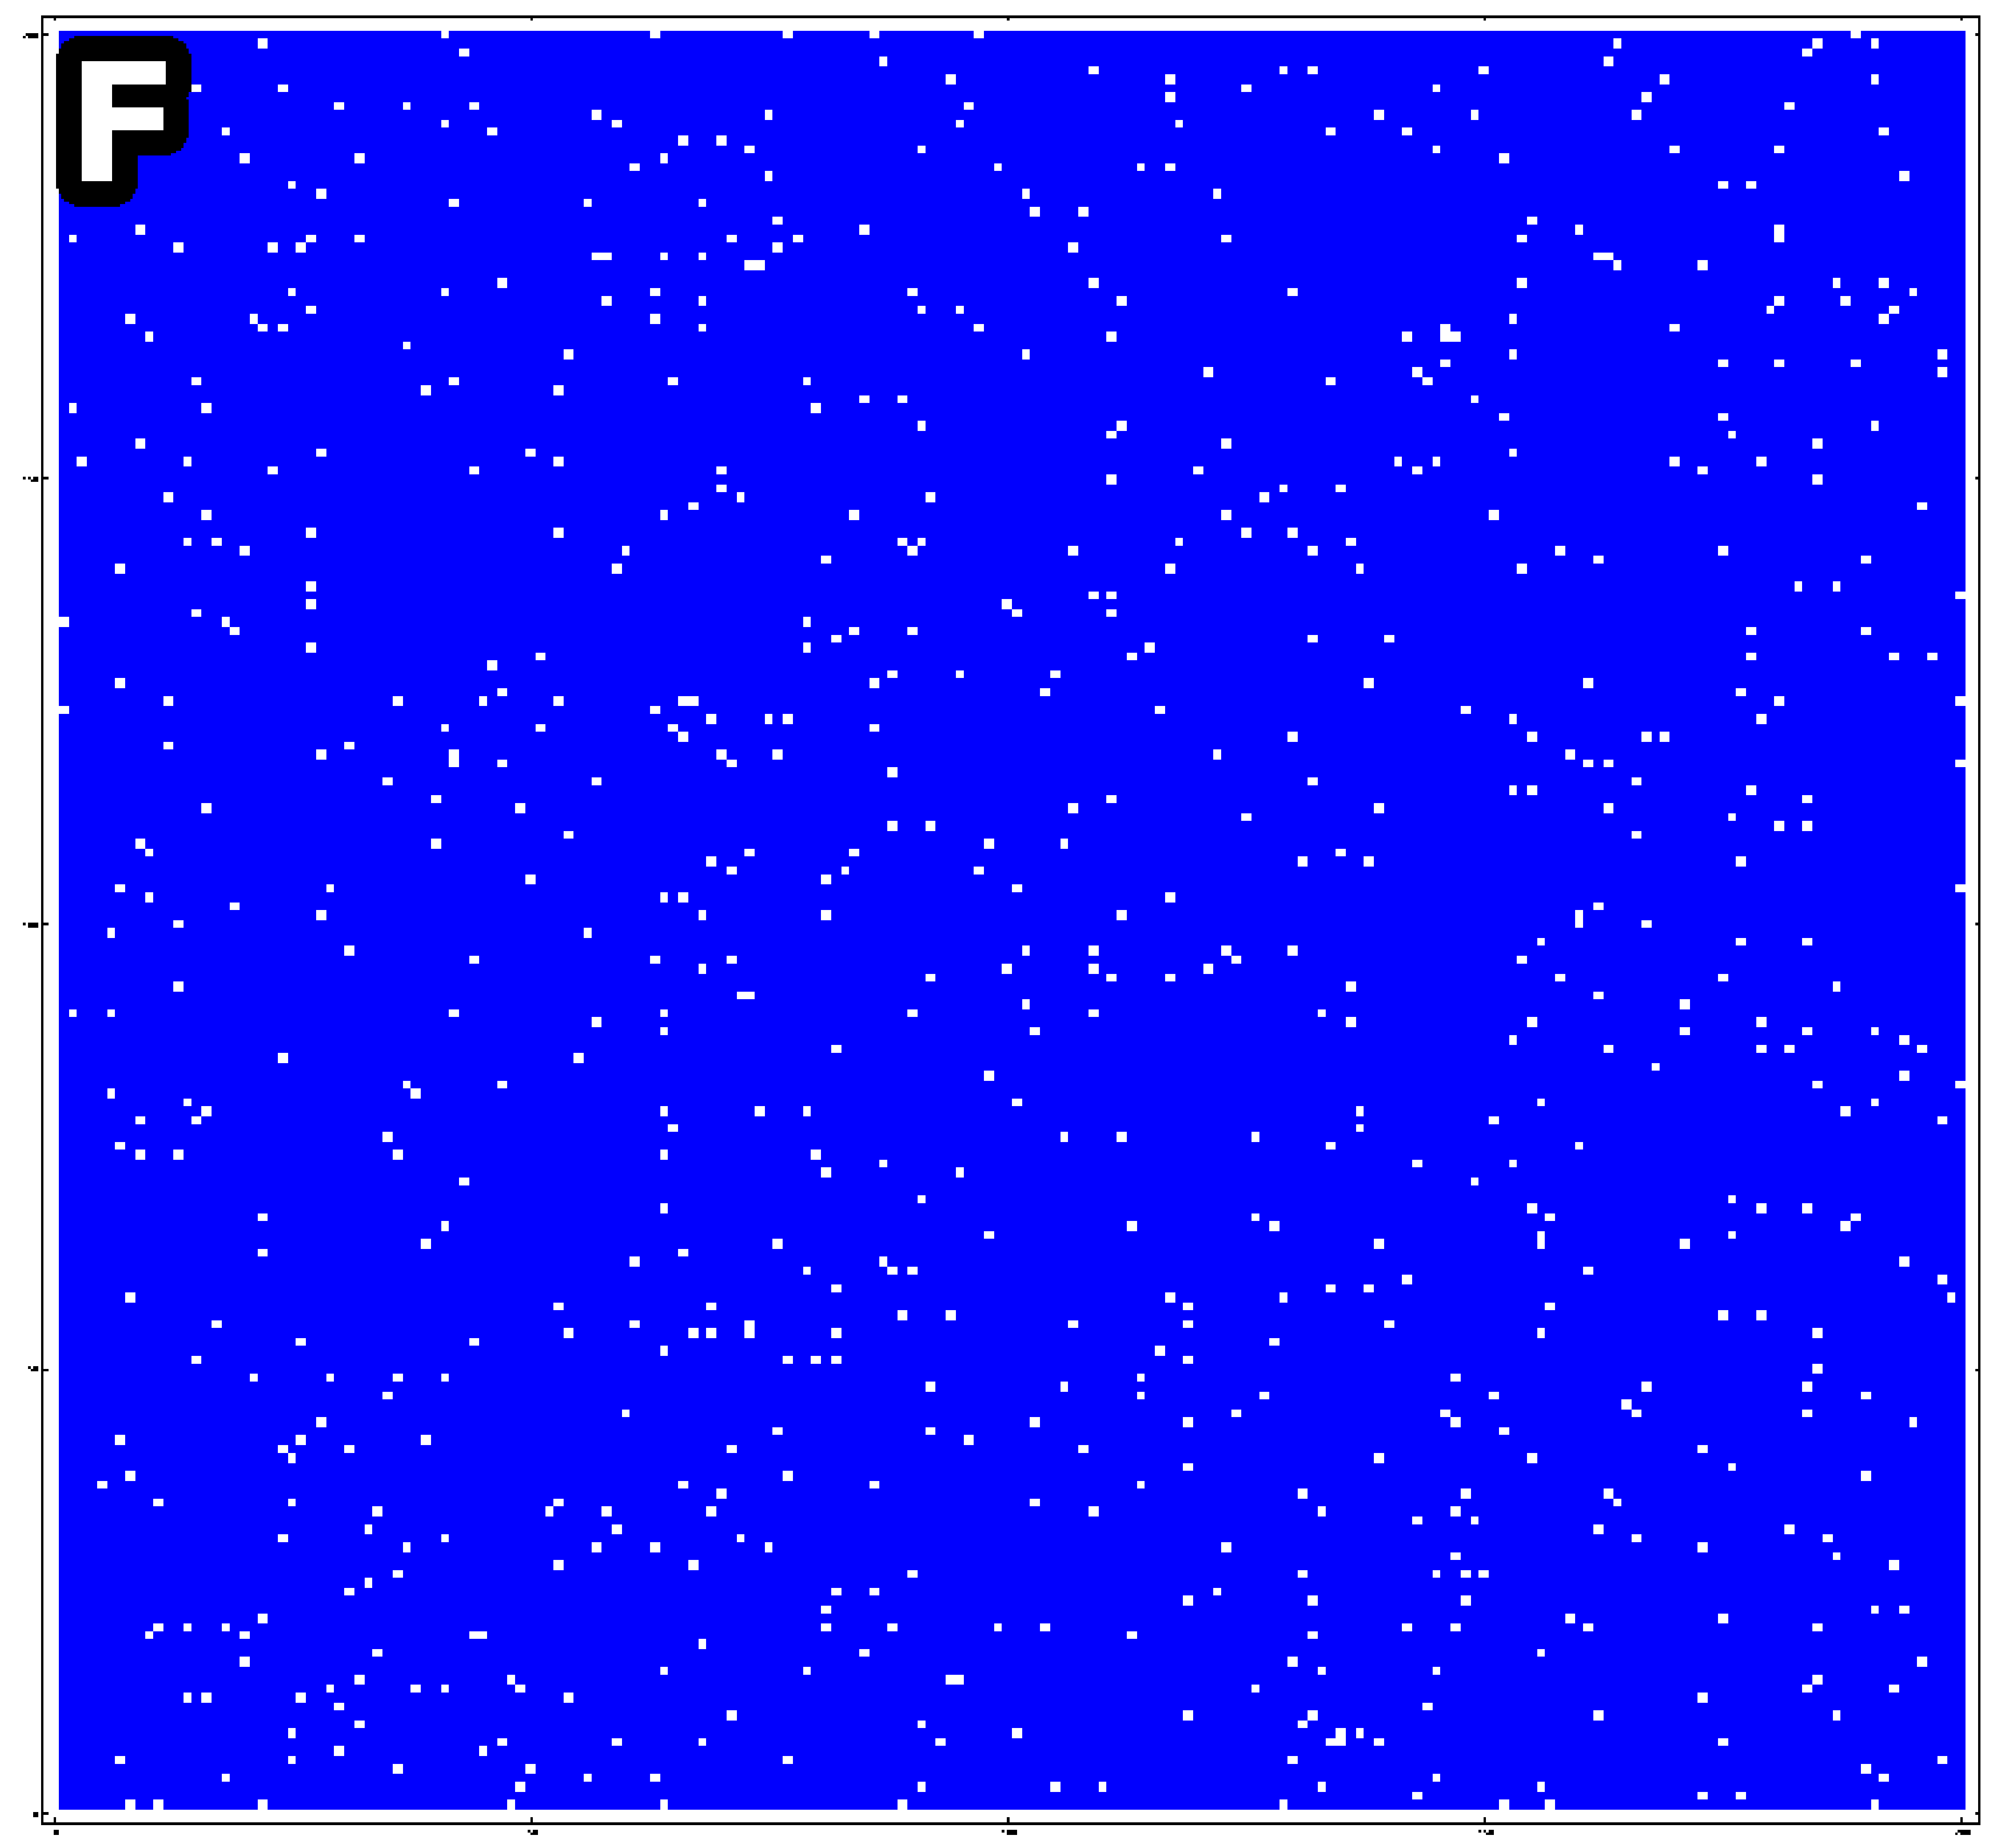
\includegraphics[width=0.25\textwidth]{imgs/0_021_heat74.eps}
%    \end{figure}
%    \vfill
%    \begin{figure}
%      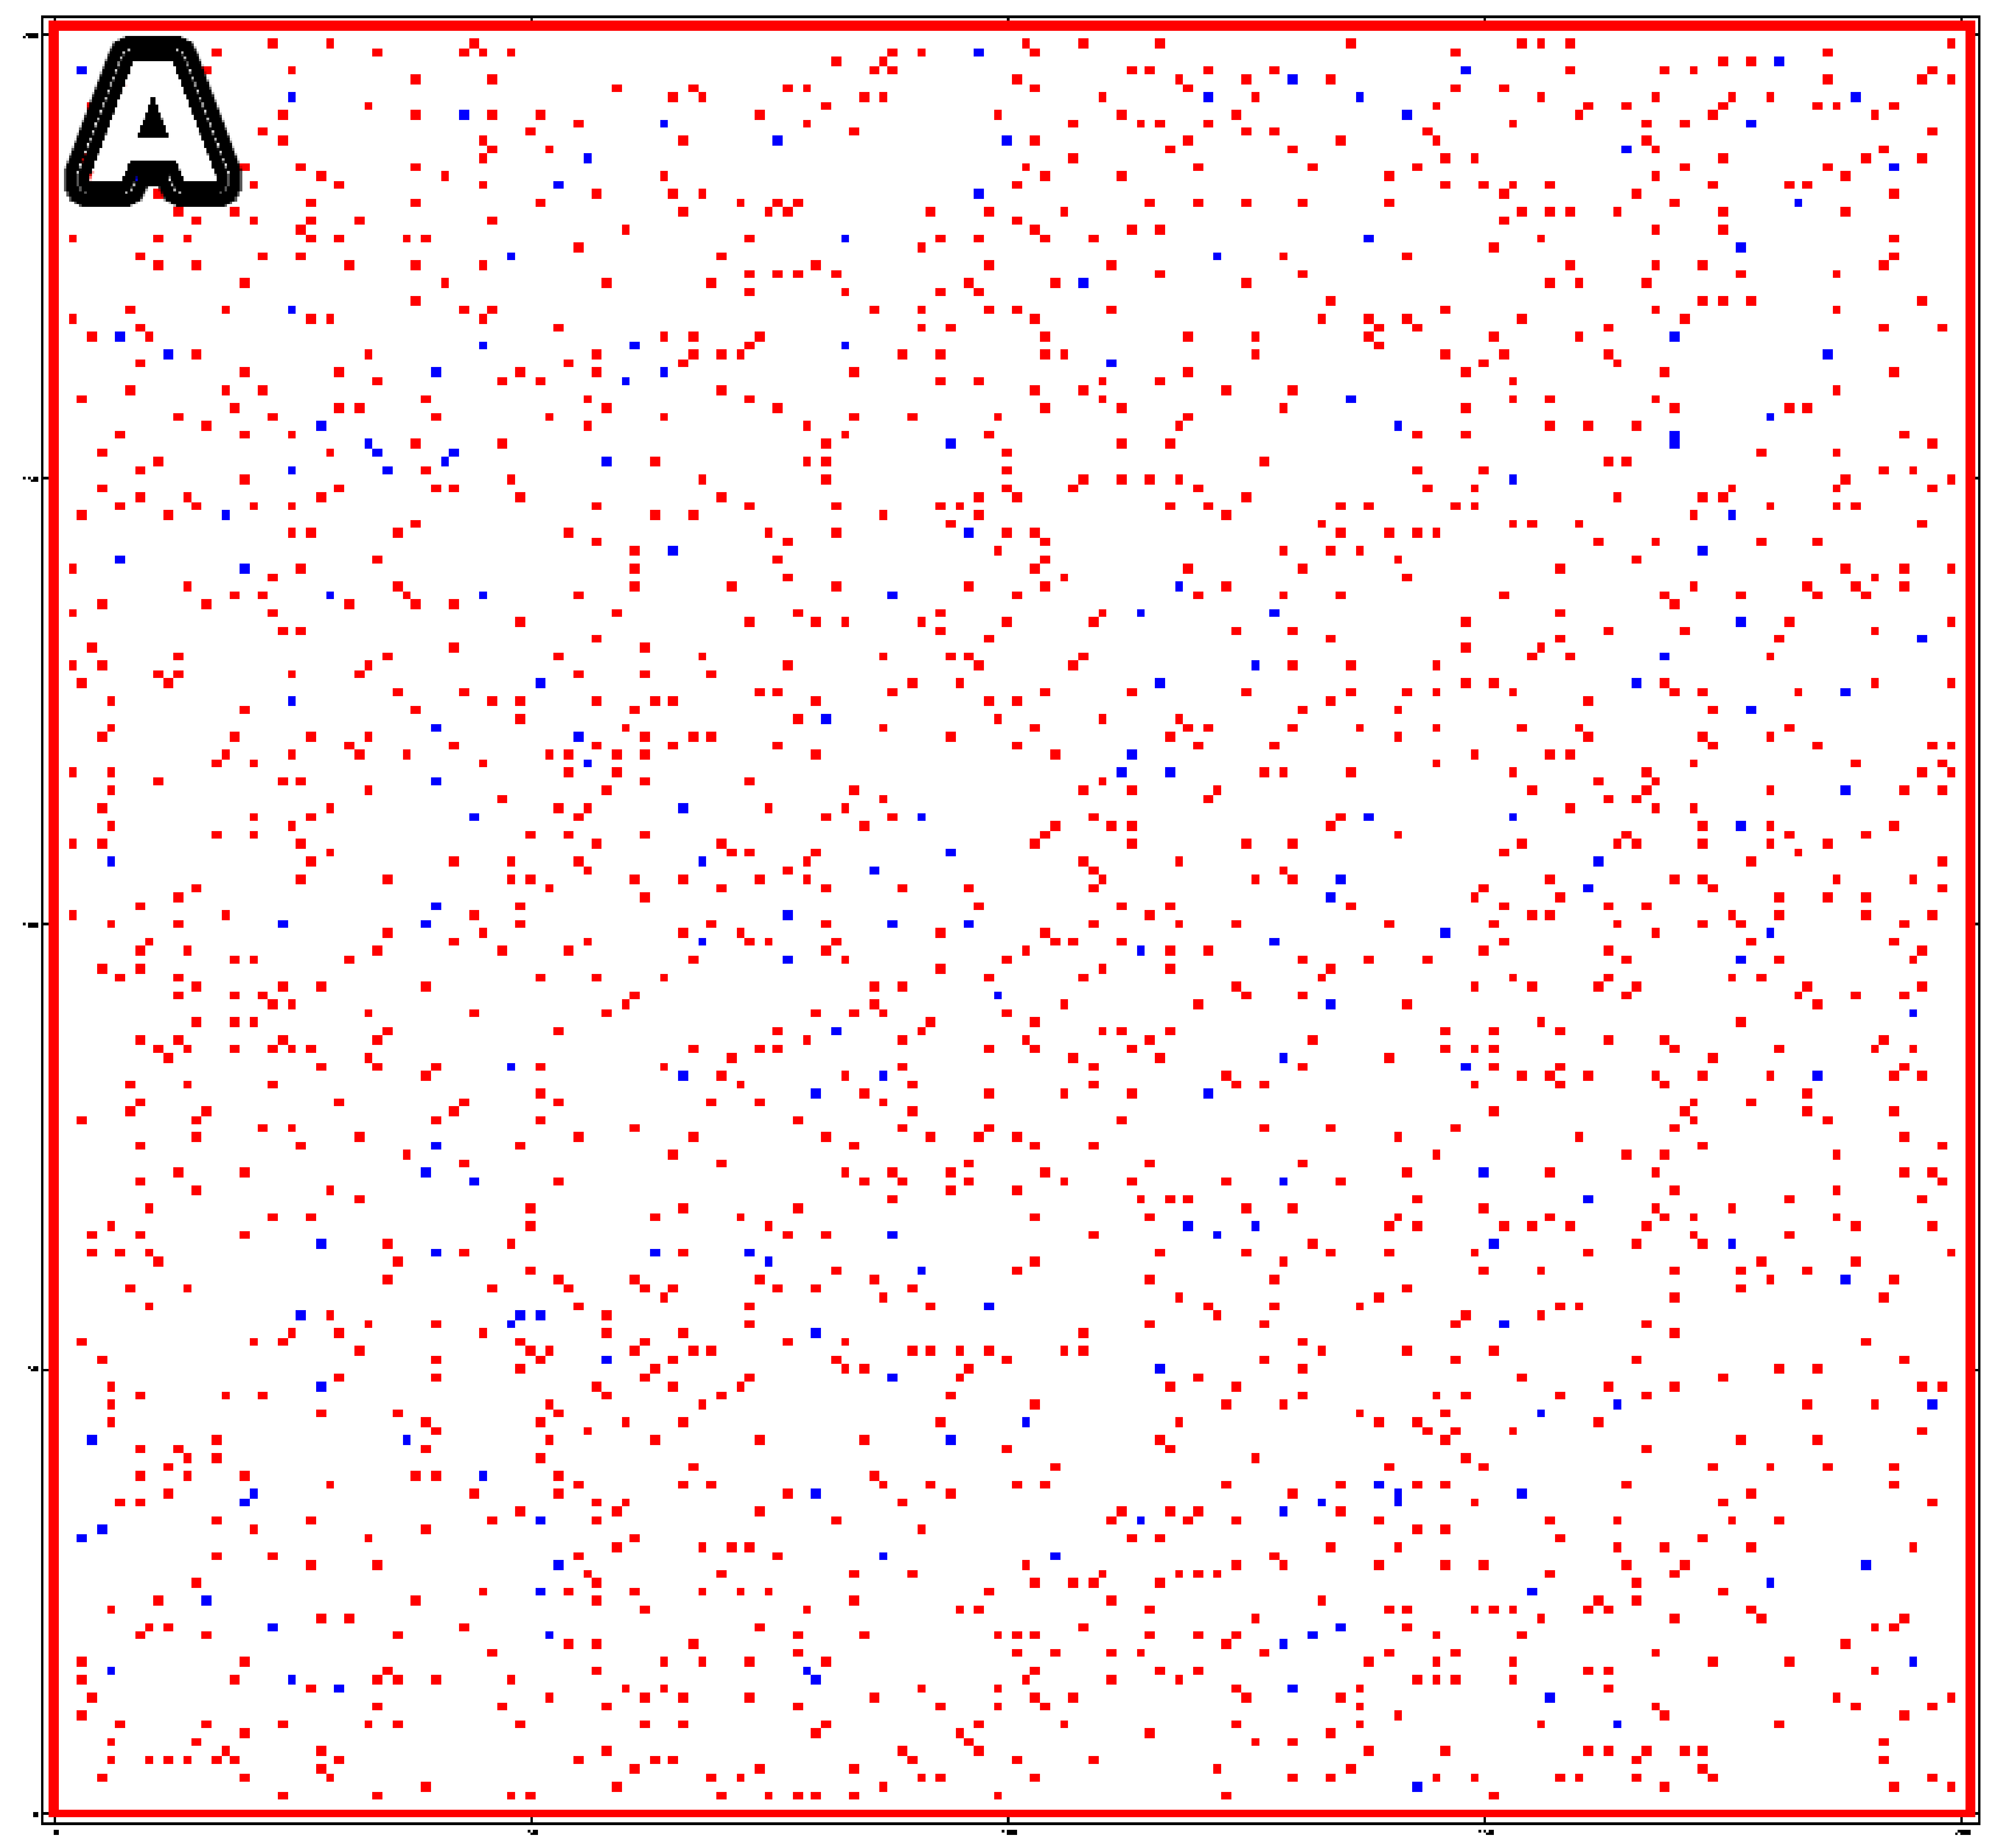
\includegraphics[width=0.25\textwidth]{imgs/2_021_heat1.eps}
%      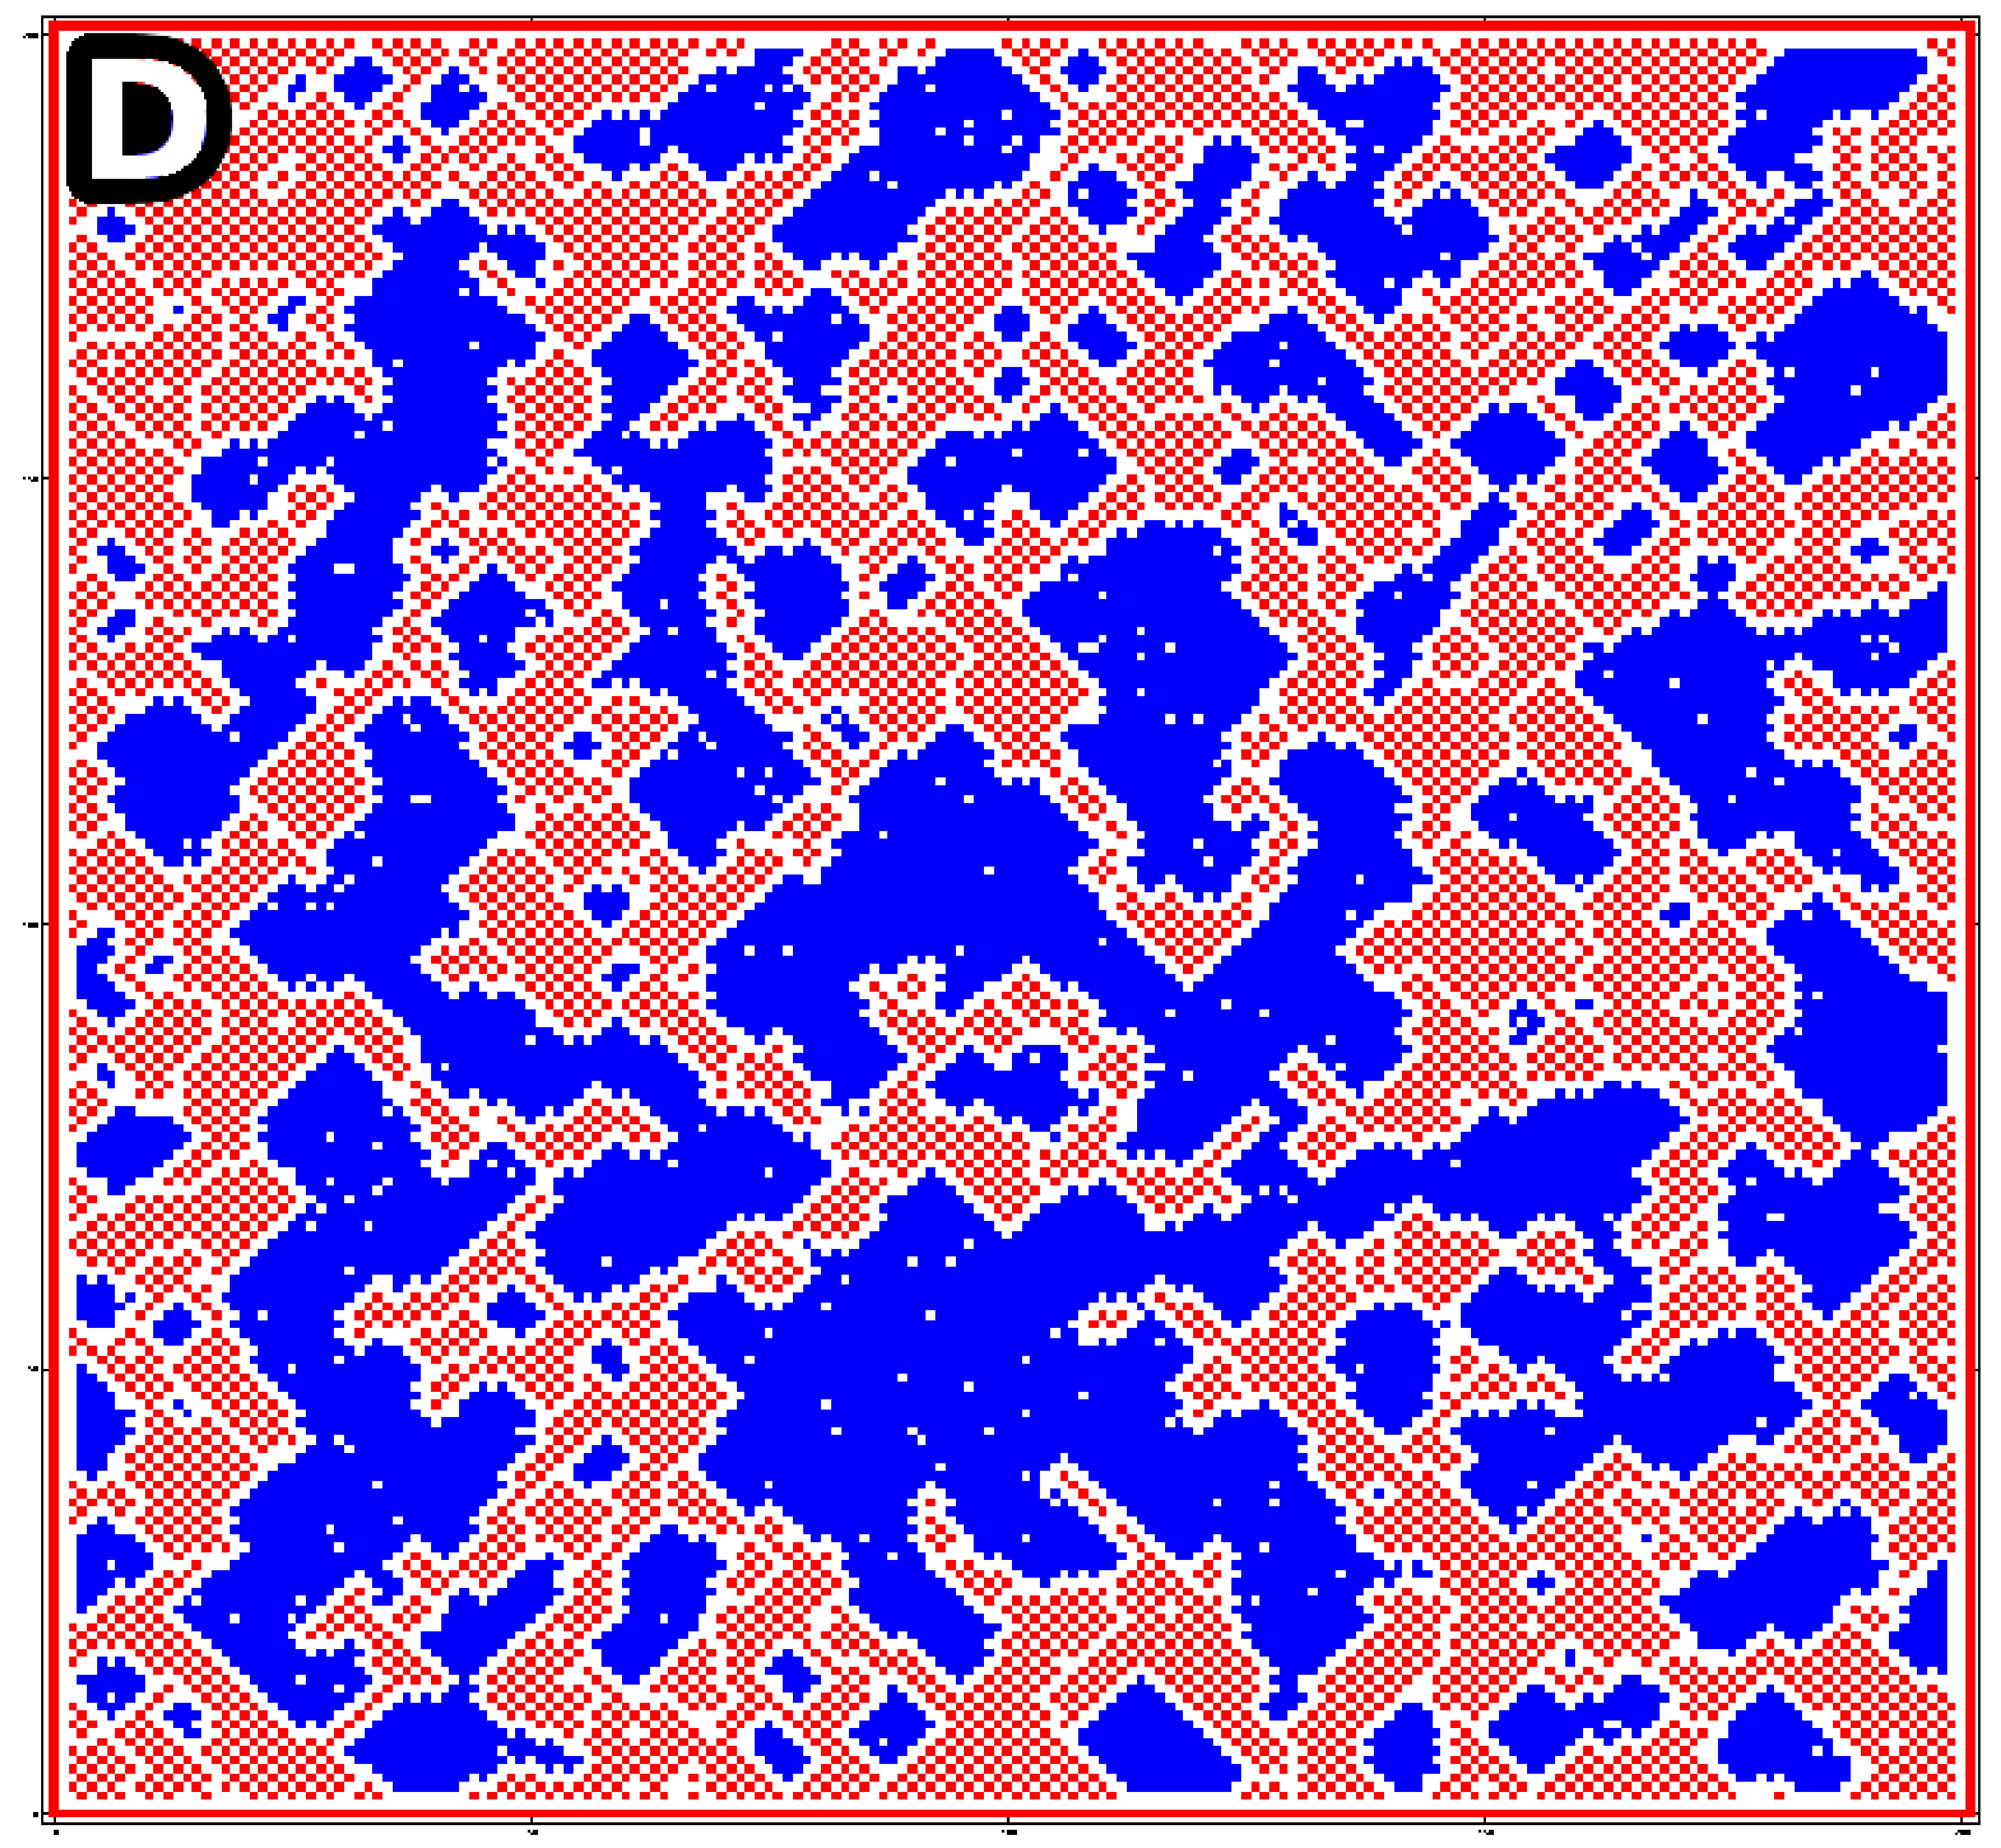
\includegraphics[width=0.25\textwidth]{imgs/2_021_heat64.eps}
%      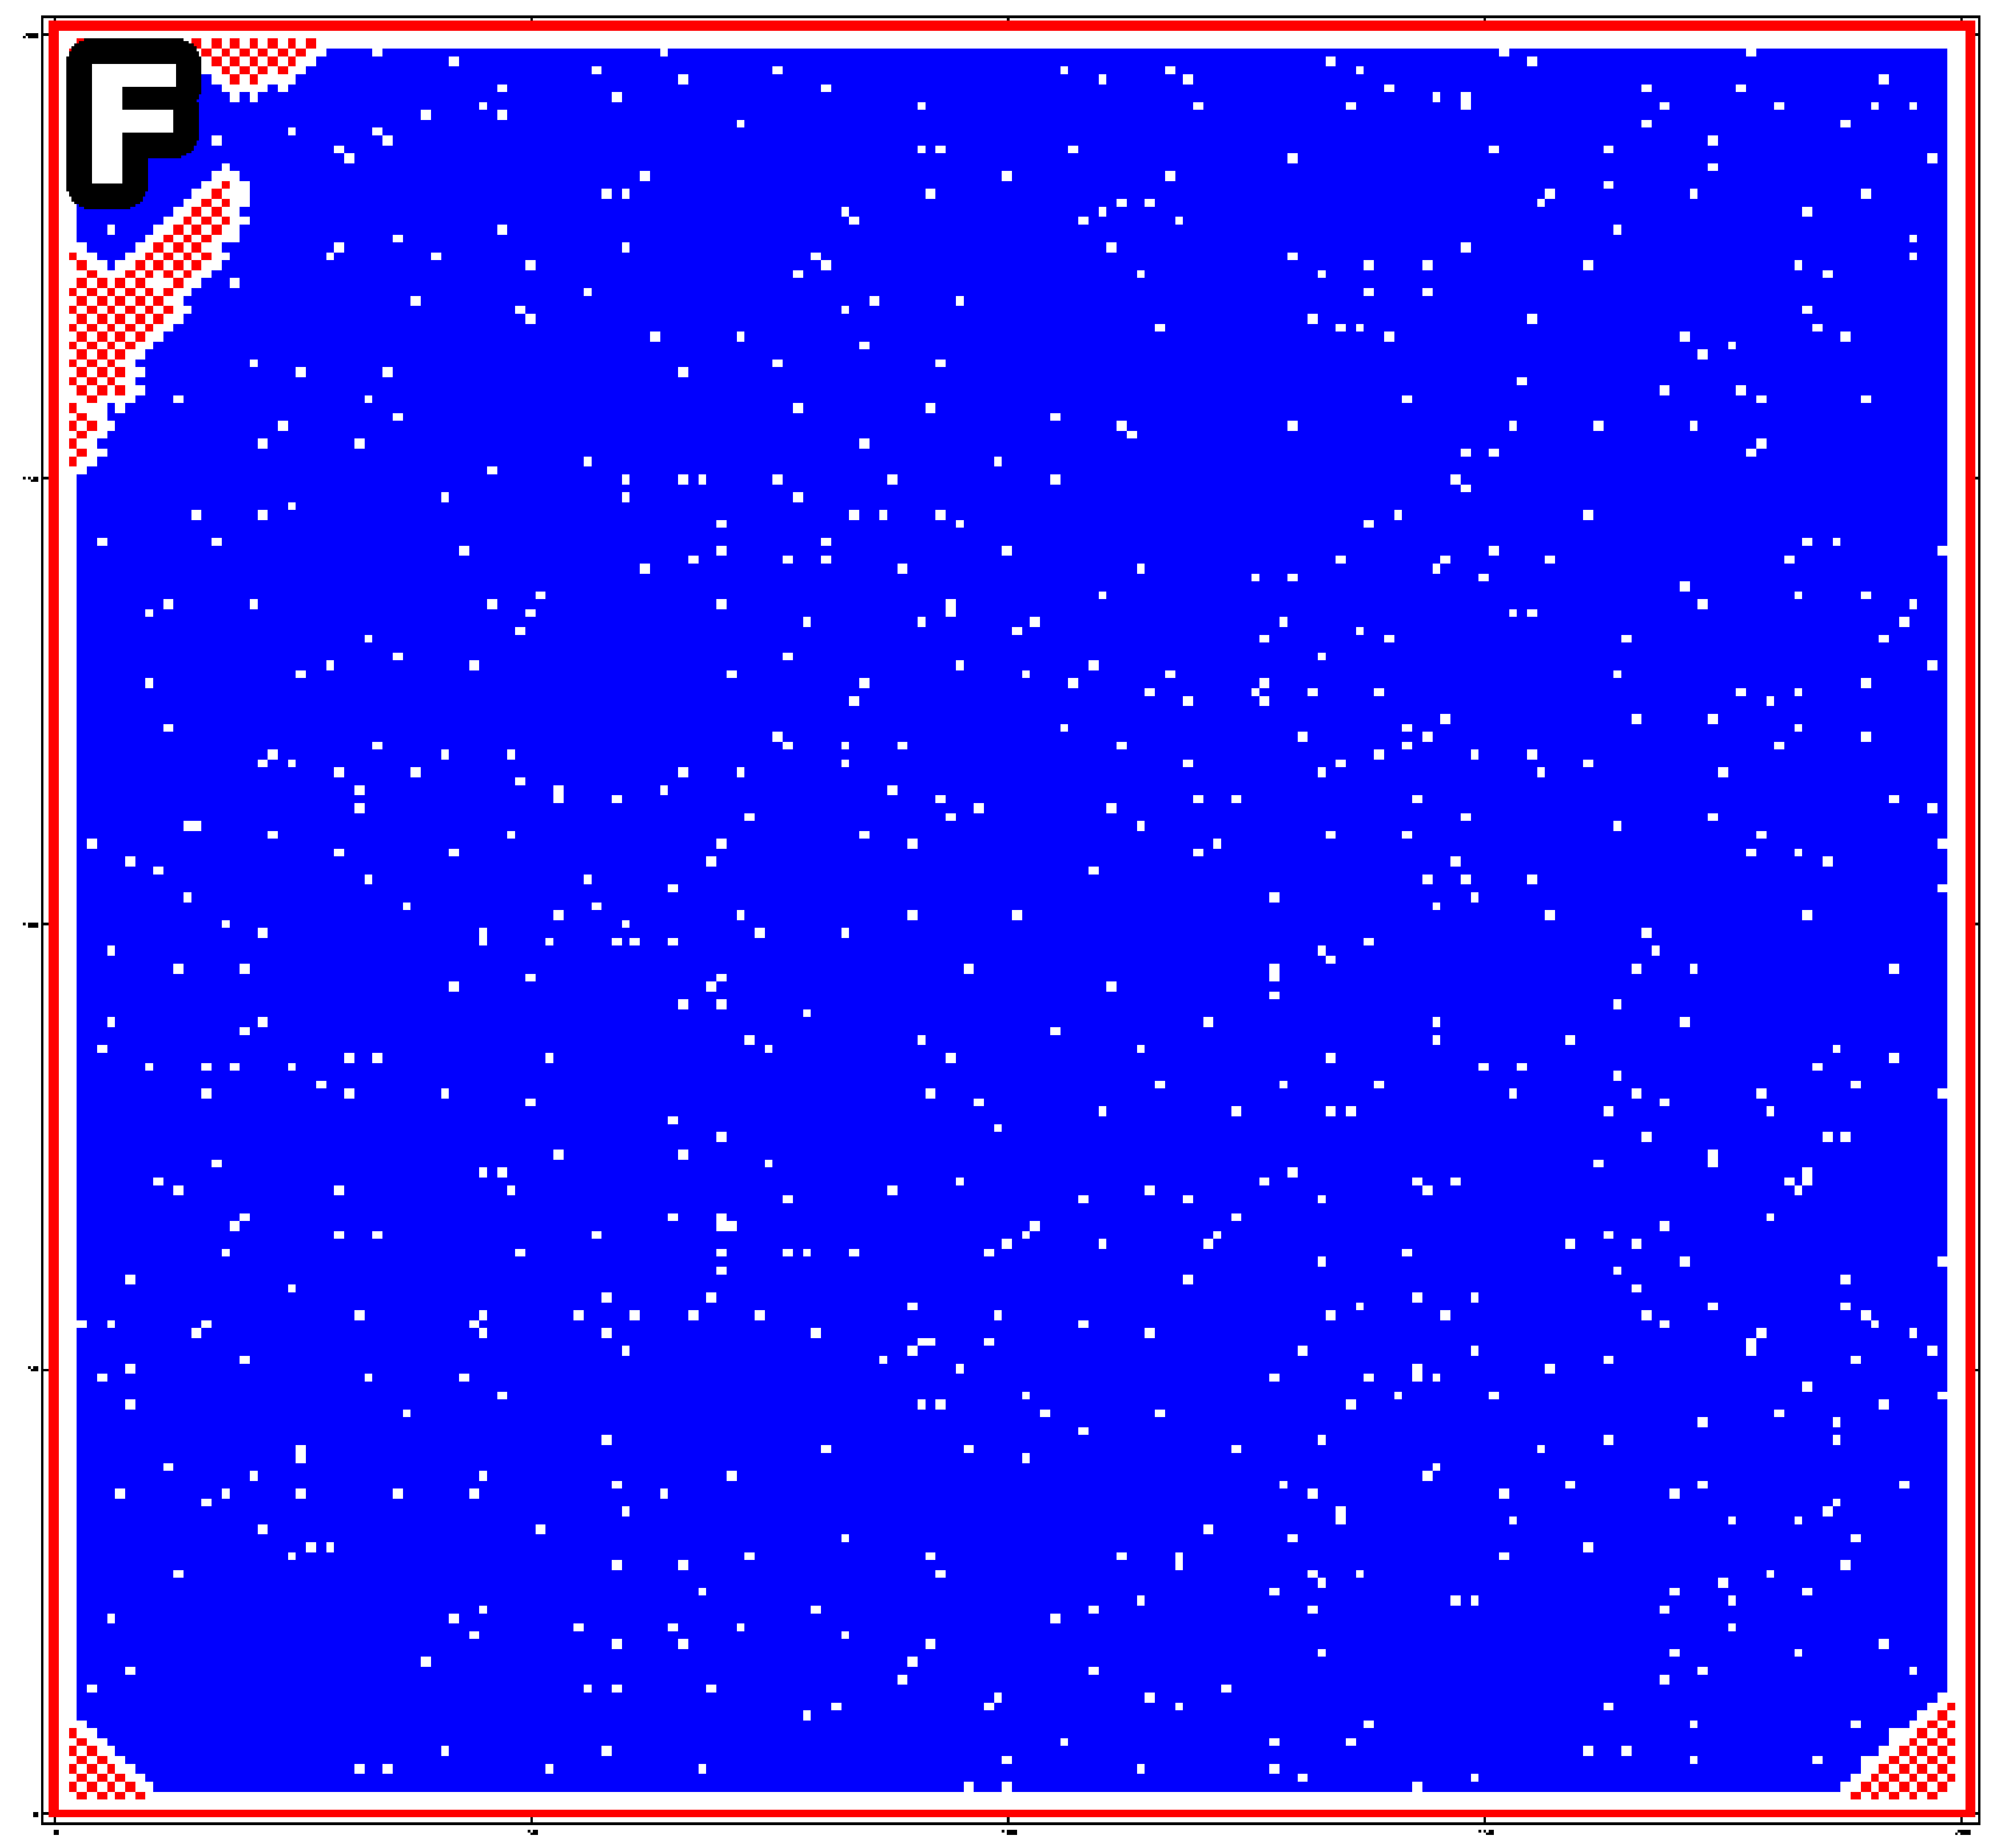
\includegraphics[width=0.25\textwidth]{imgs/2_021_heat74.eps}
%    \end{figure}
%    \vfill
%    \begin{figure}
%      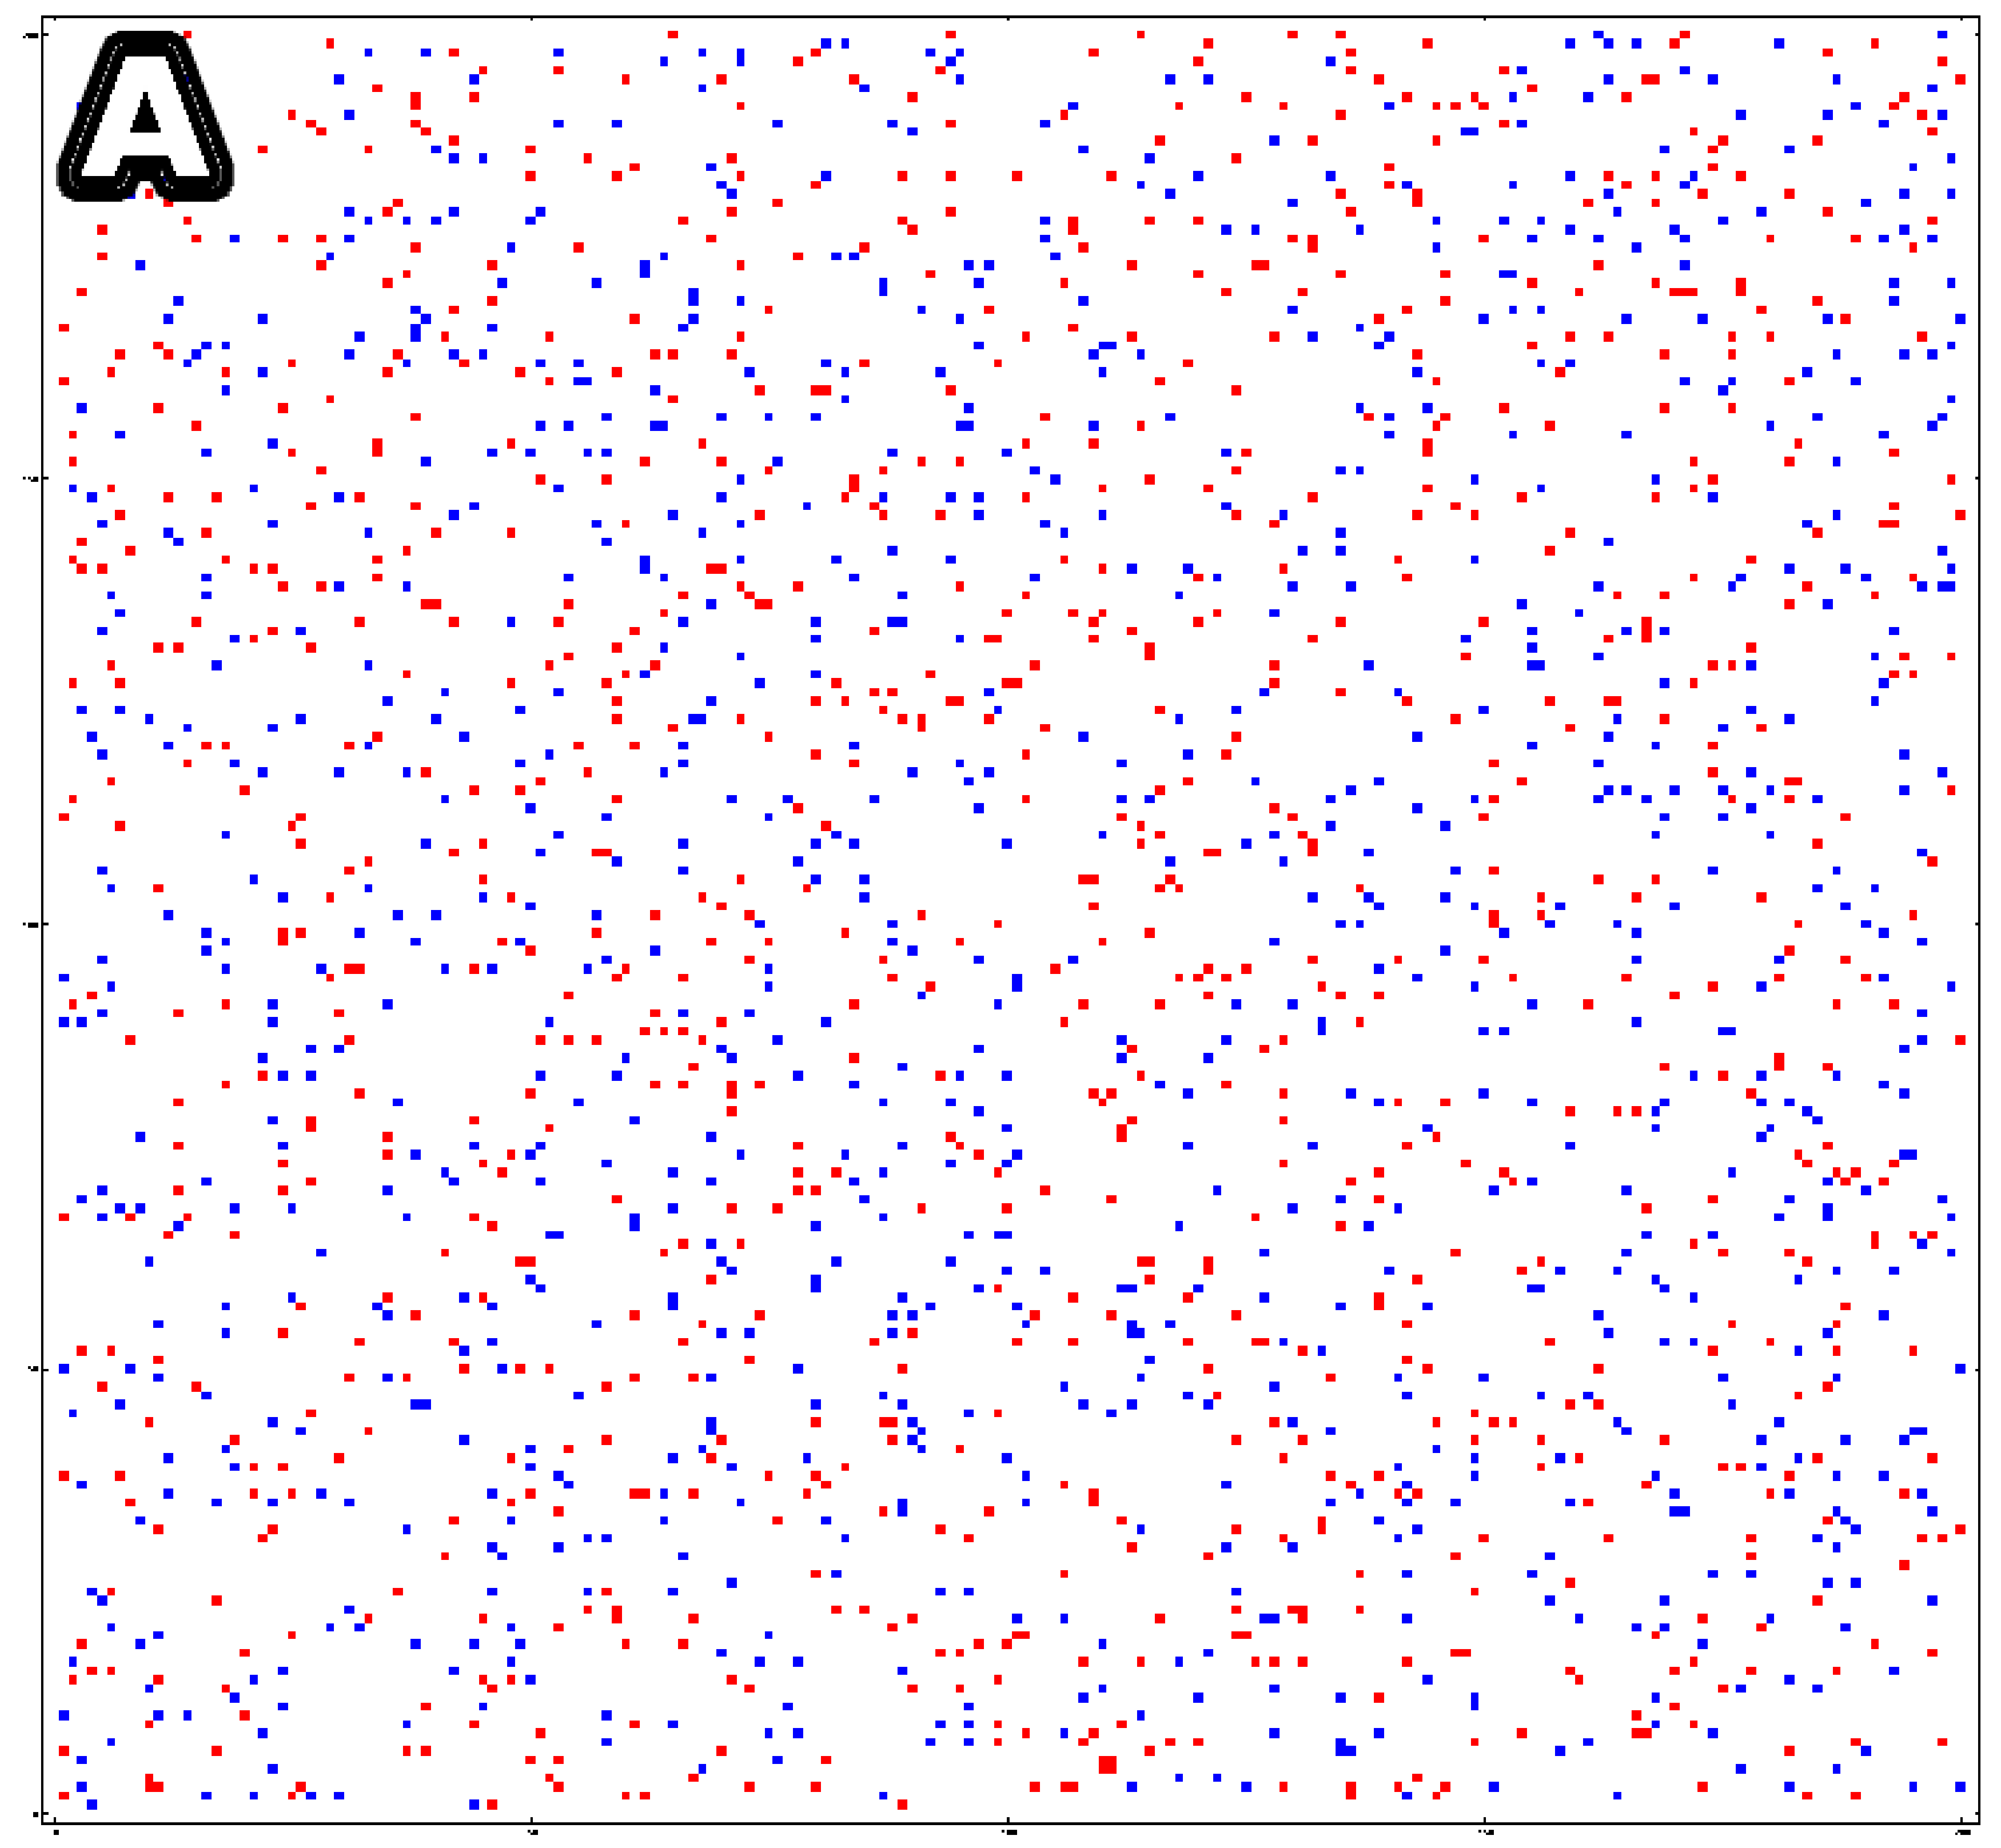
\includegraphics[width=0.25\textwidth]{imgs/01_010_heat1.eps}
%      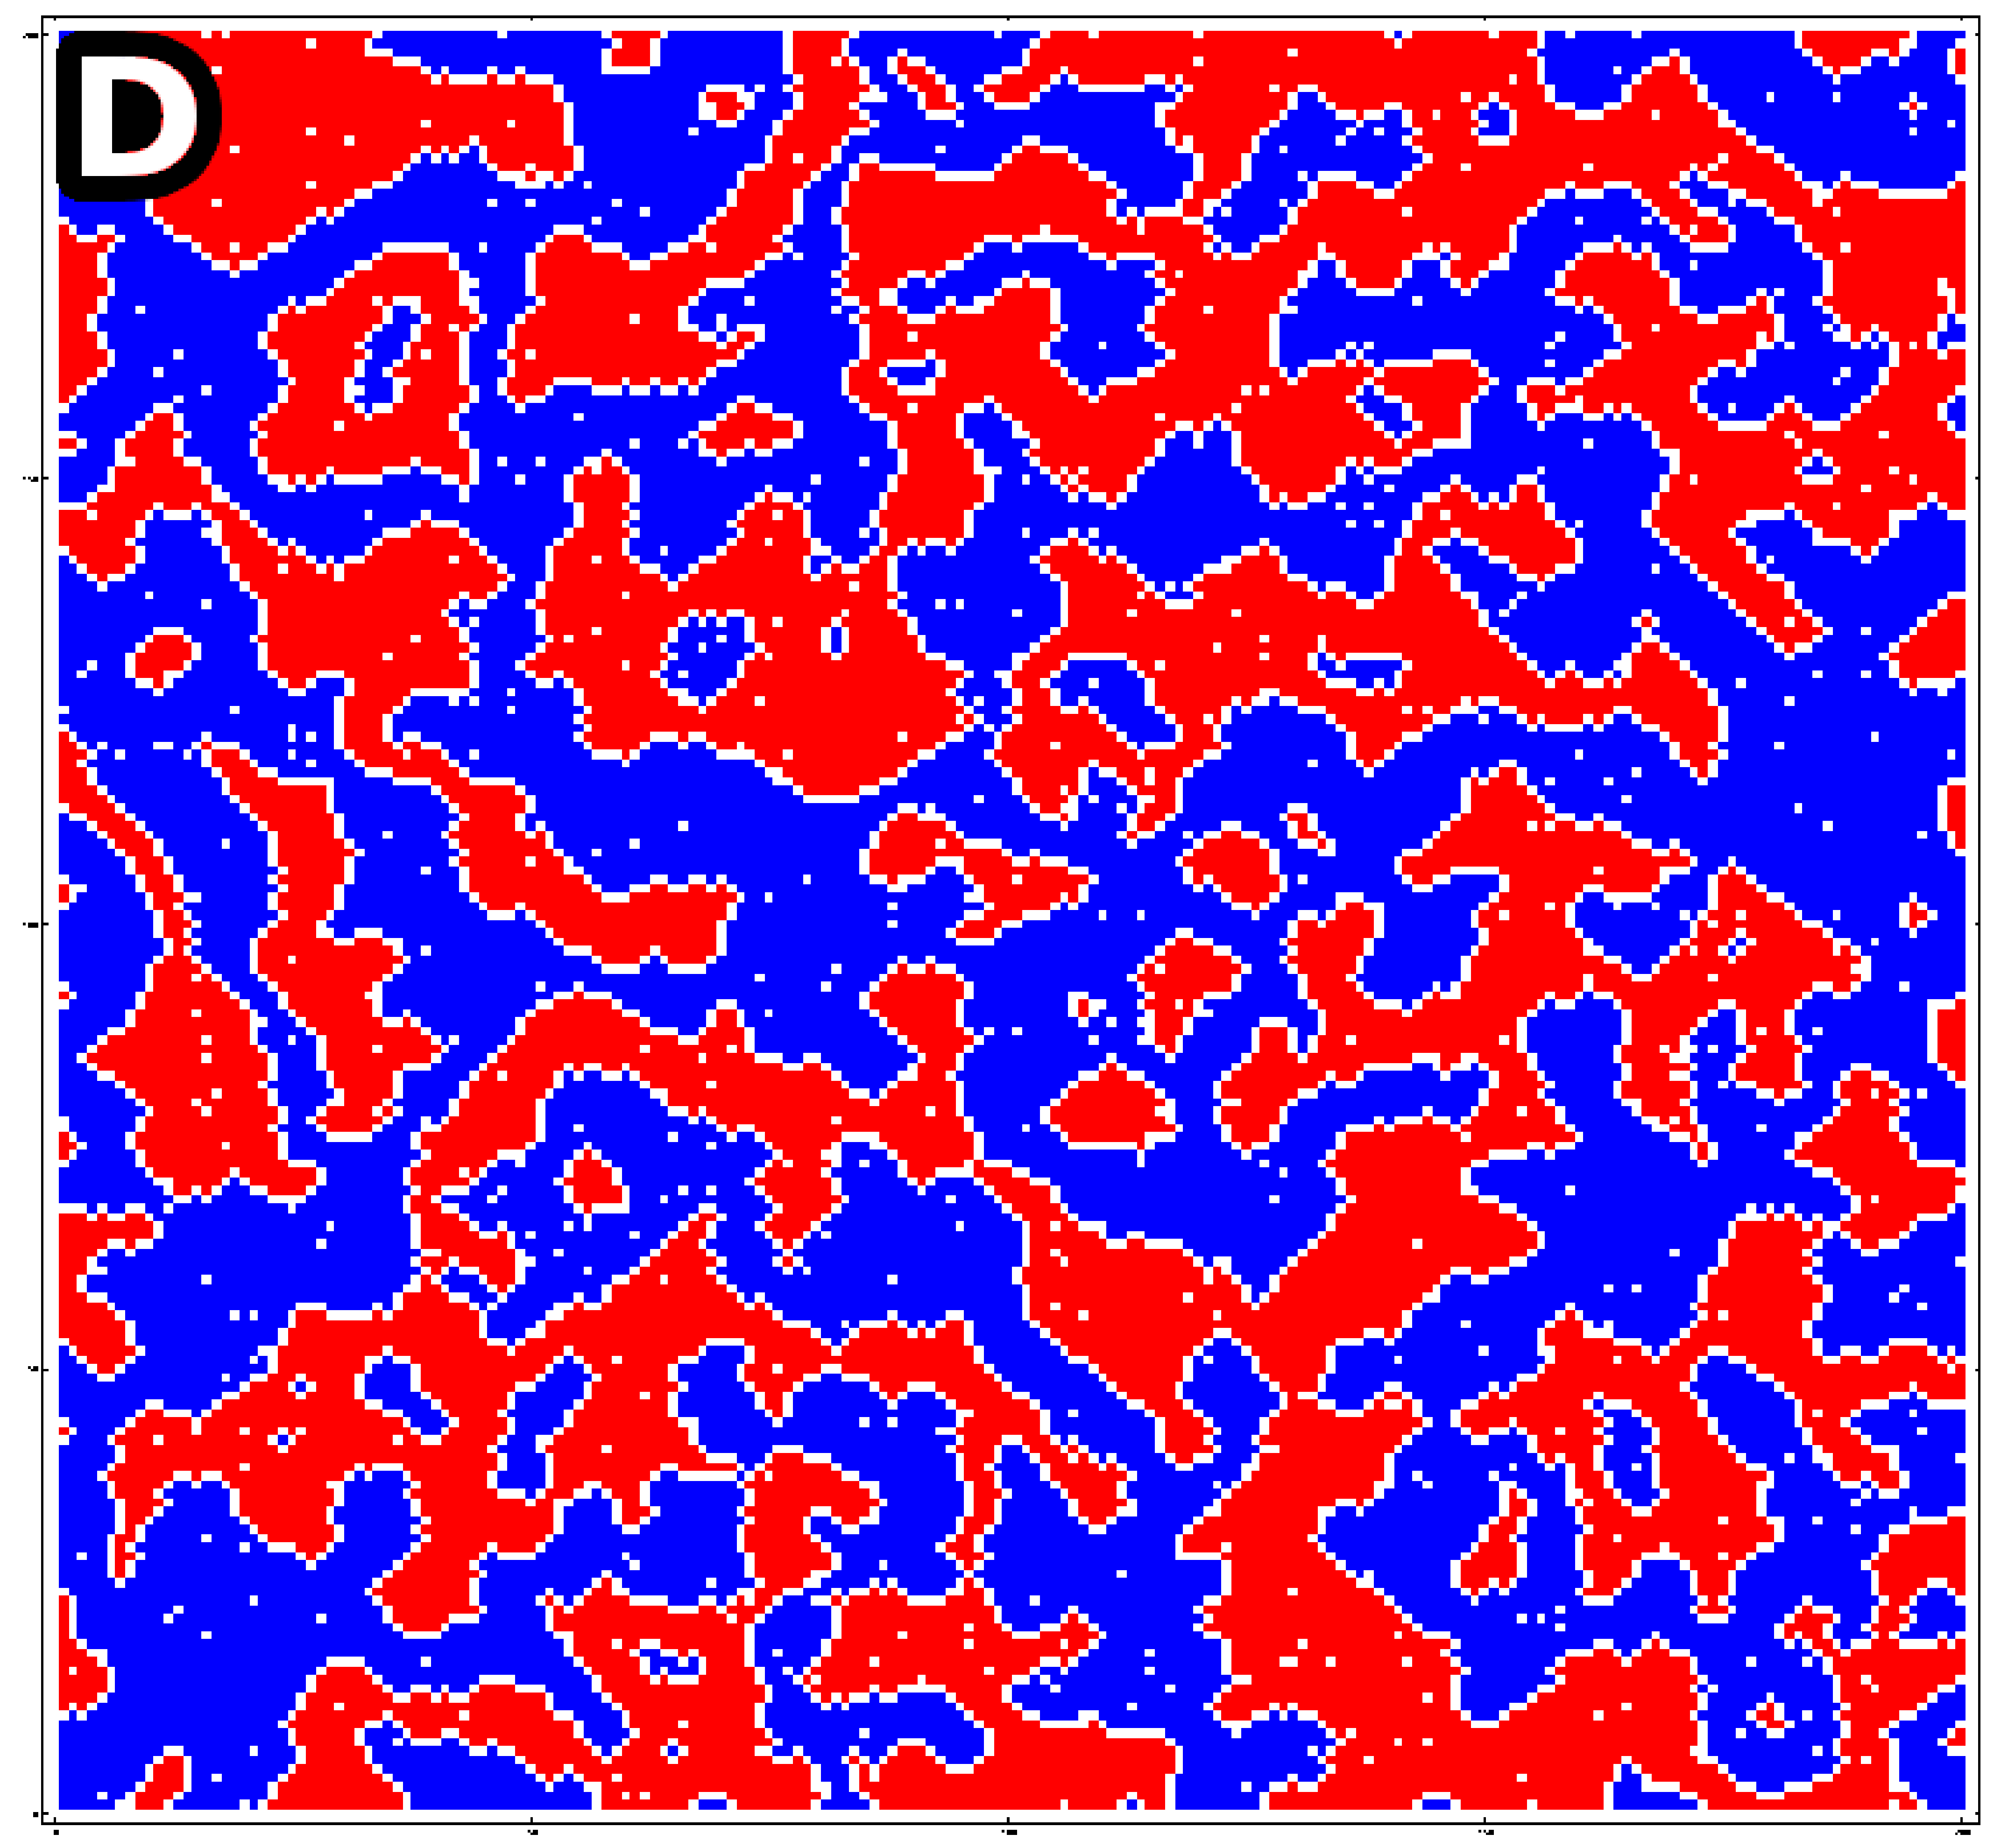
\includegraphics[width=0.25\textwidth]{imgs/01_010_heat64.eps}
%      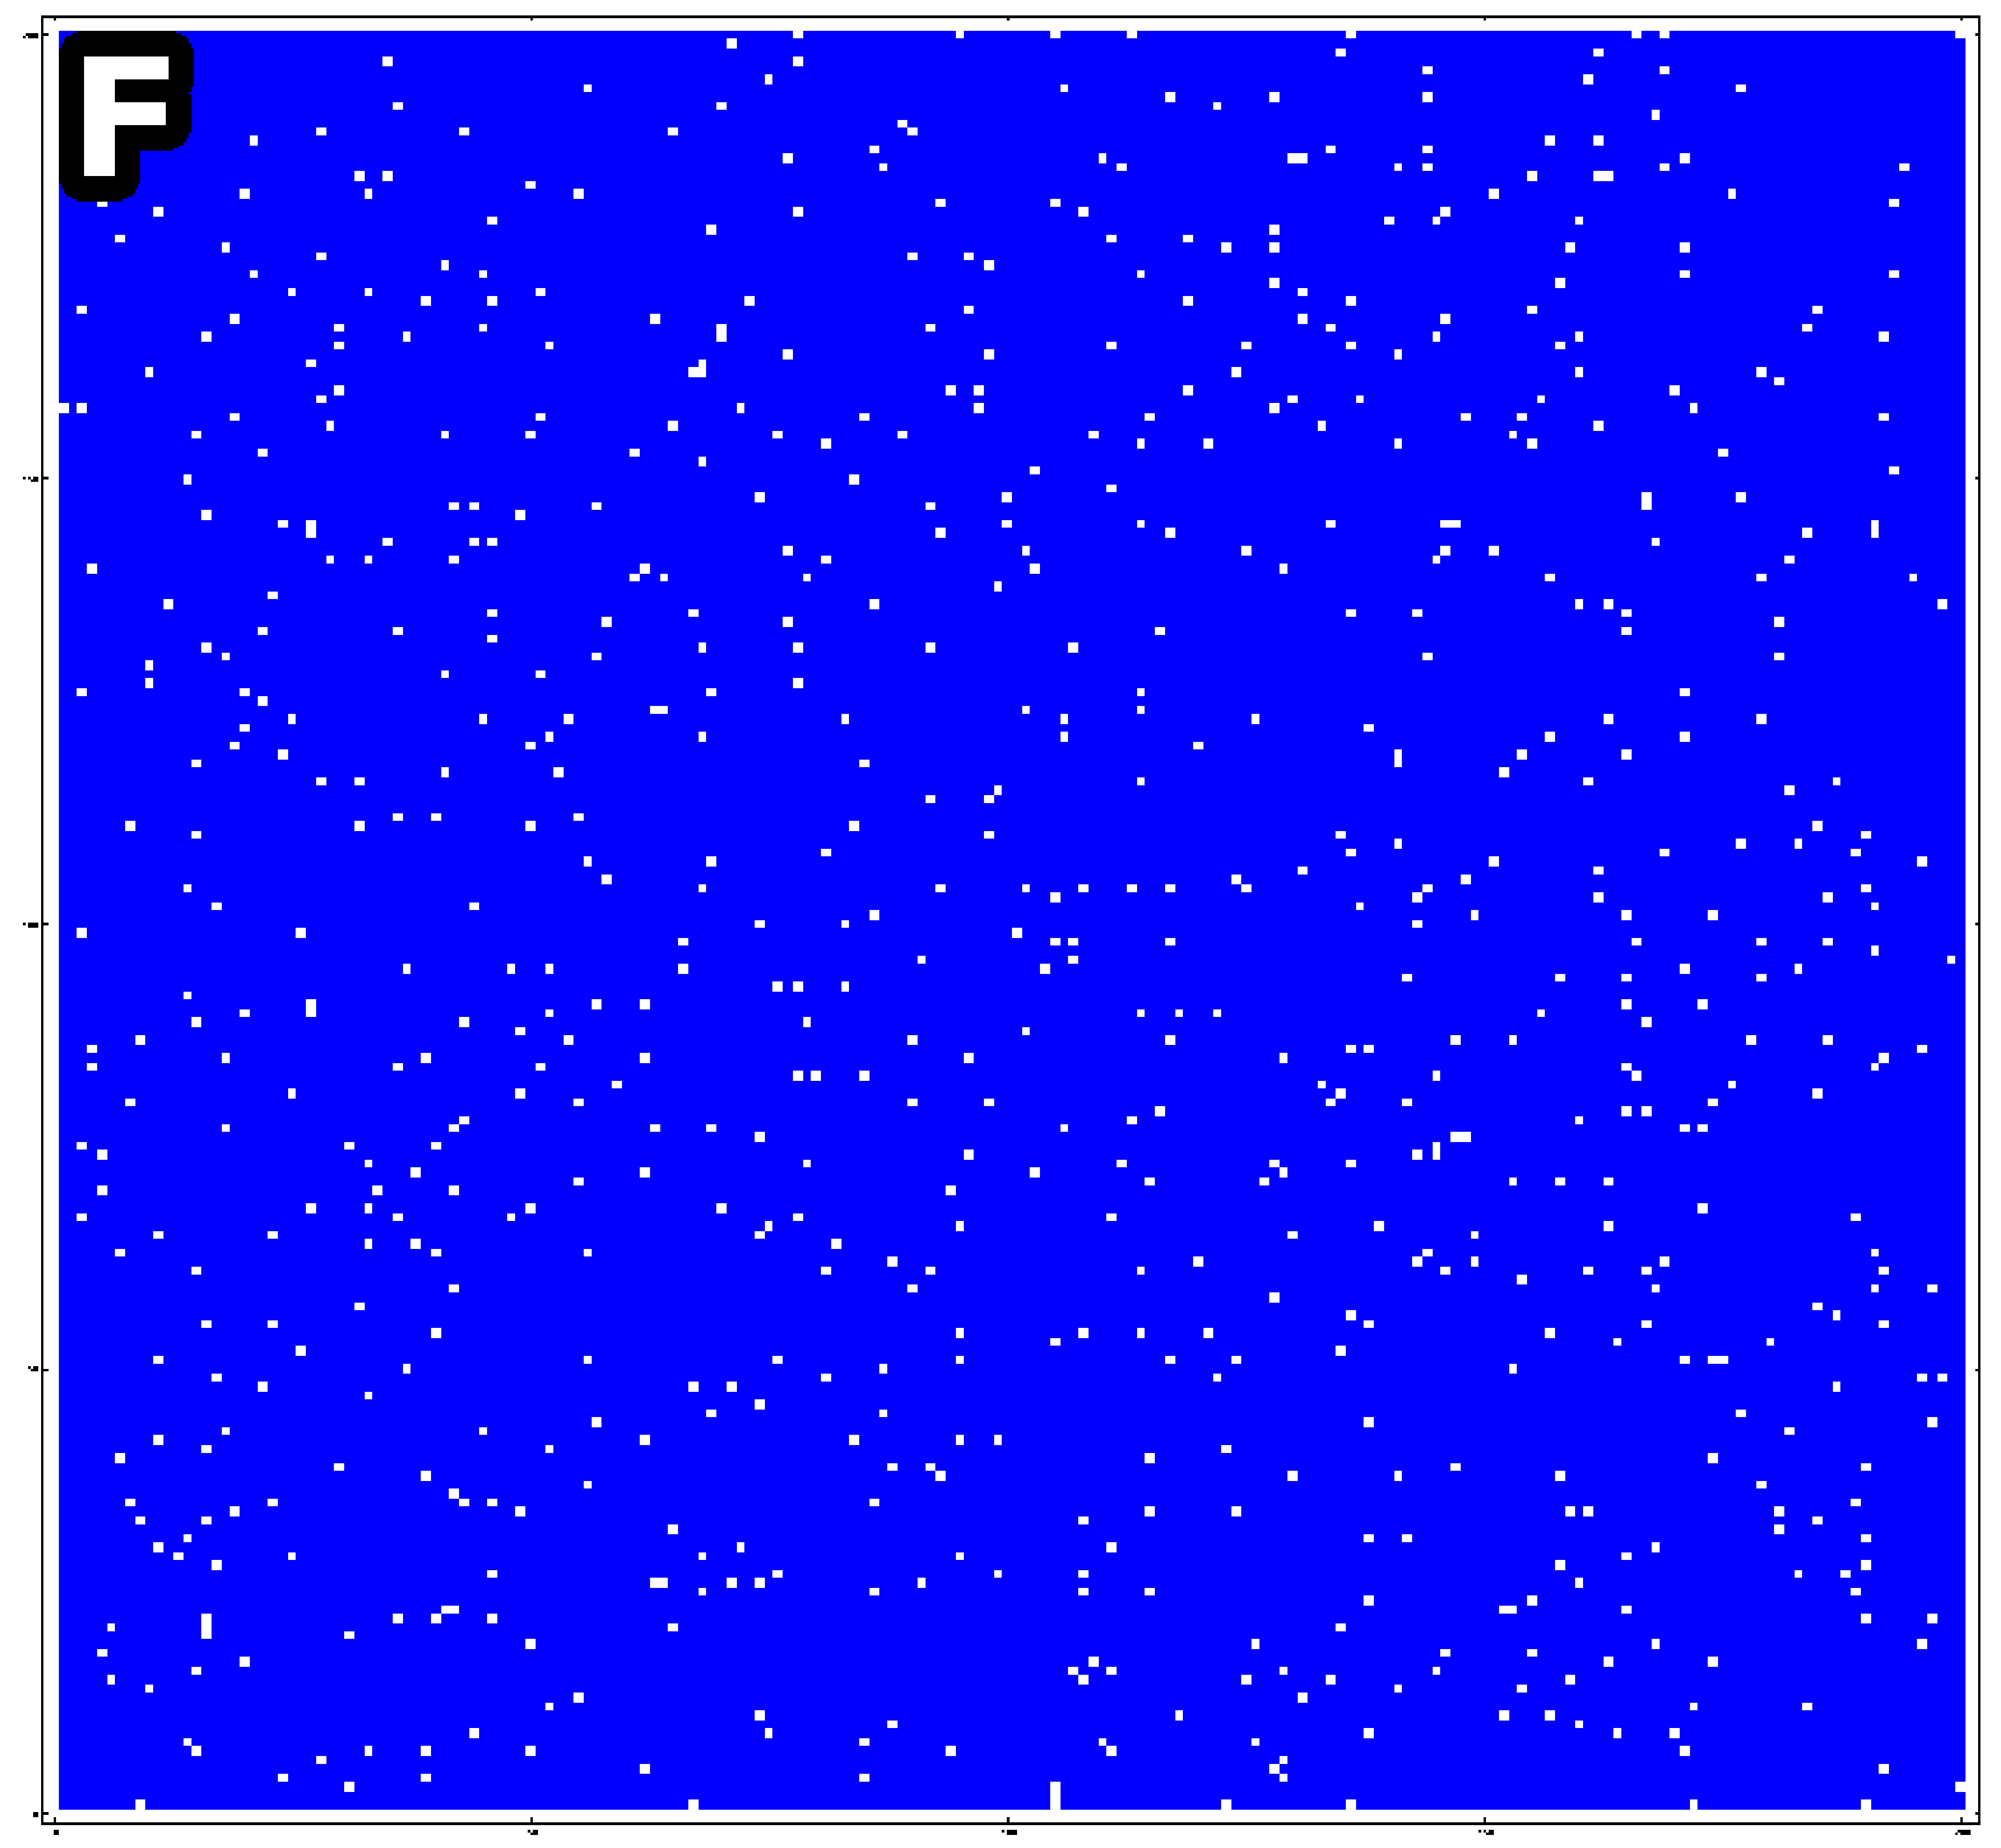
\includegraphics[width=0.25\textwidth]{imgs/01_010_heat93.eps}
%      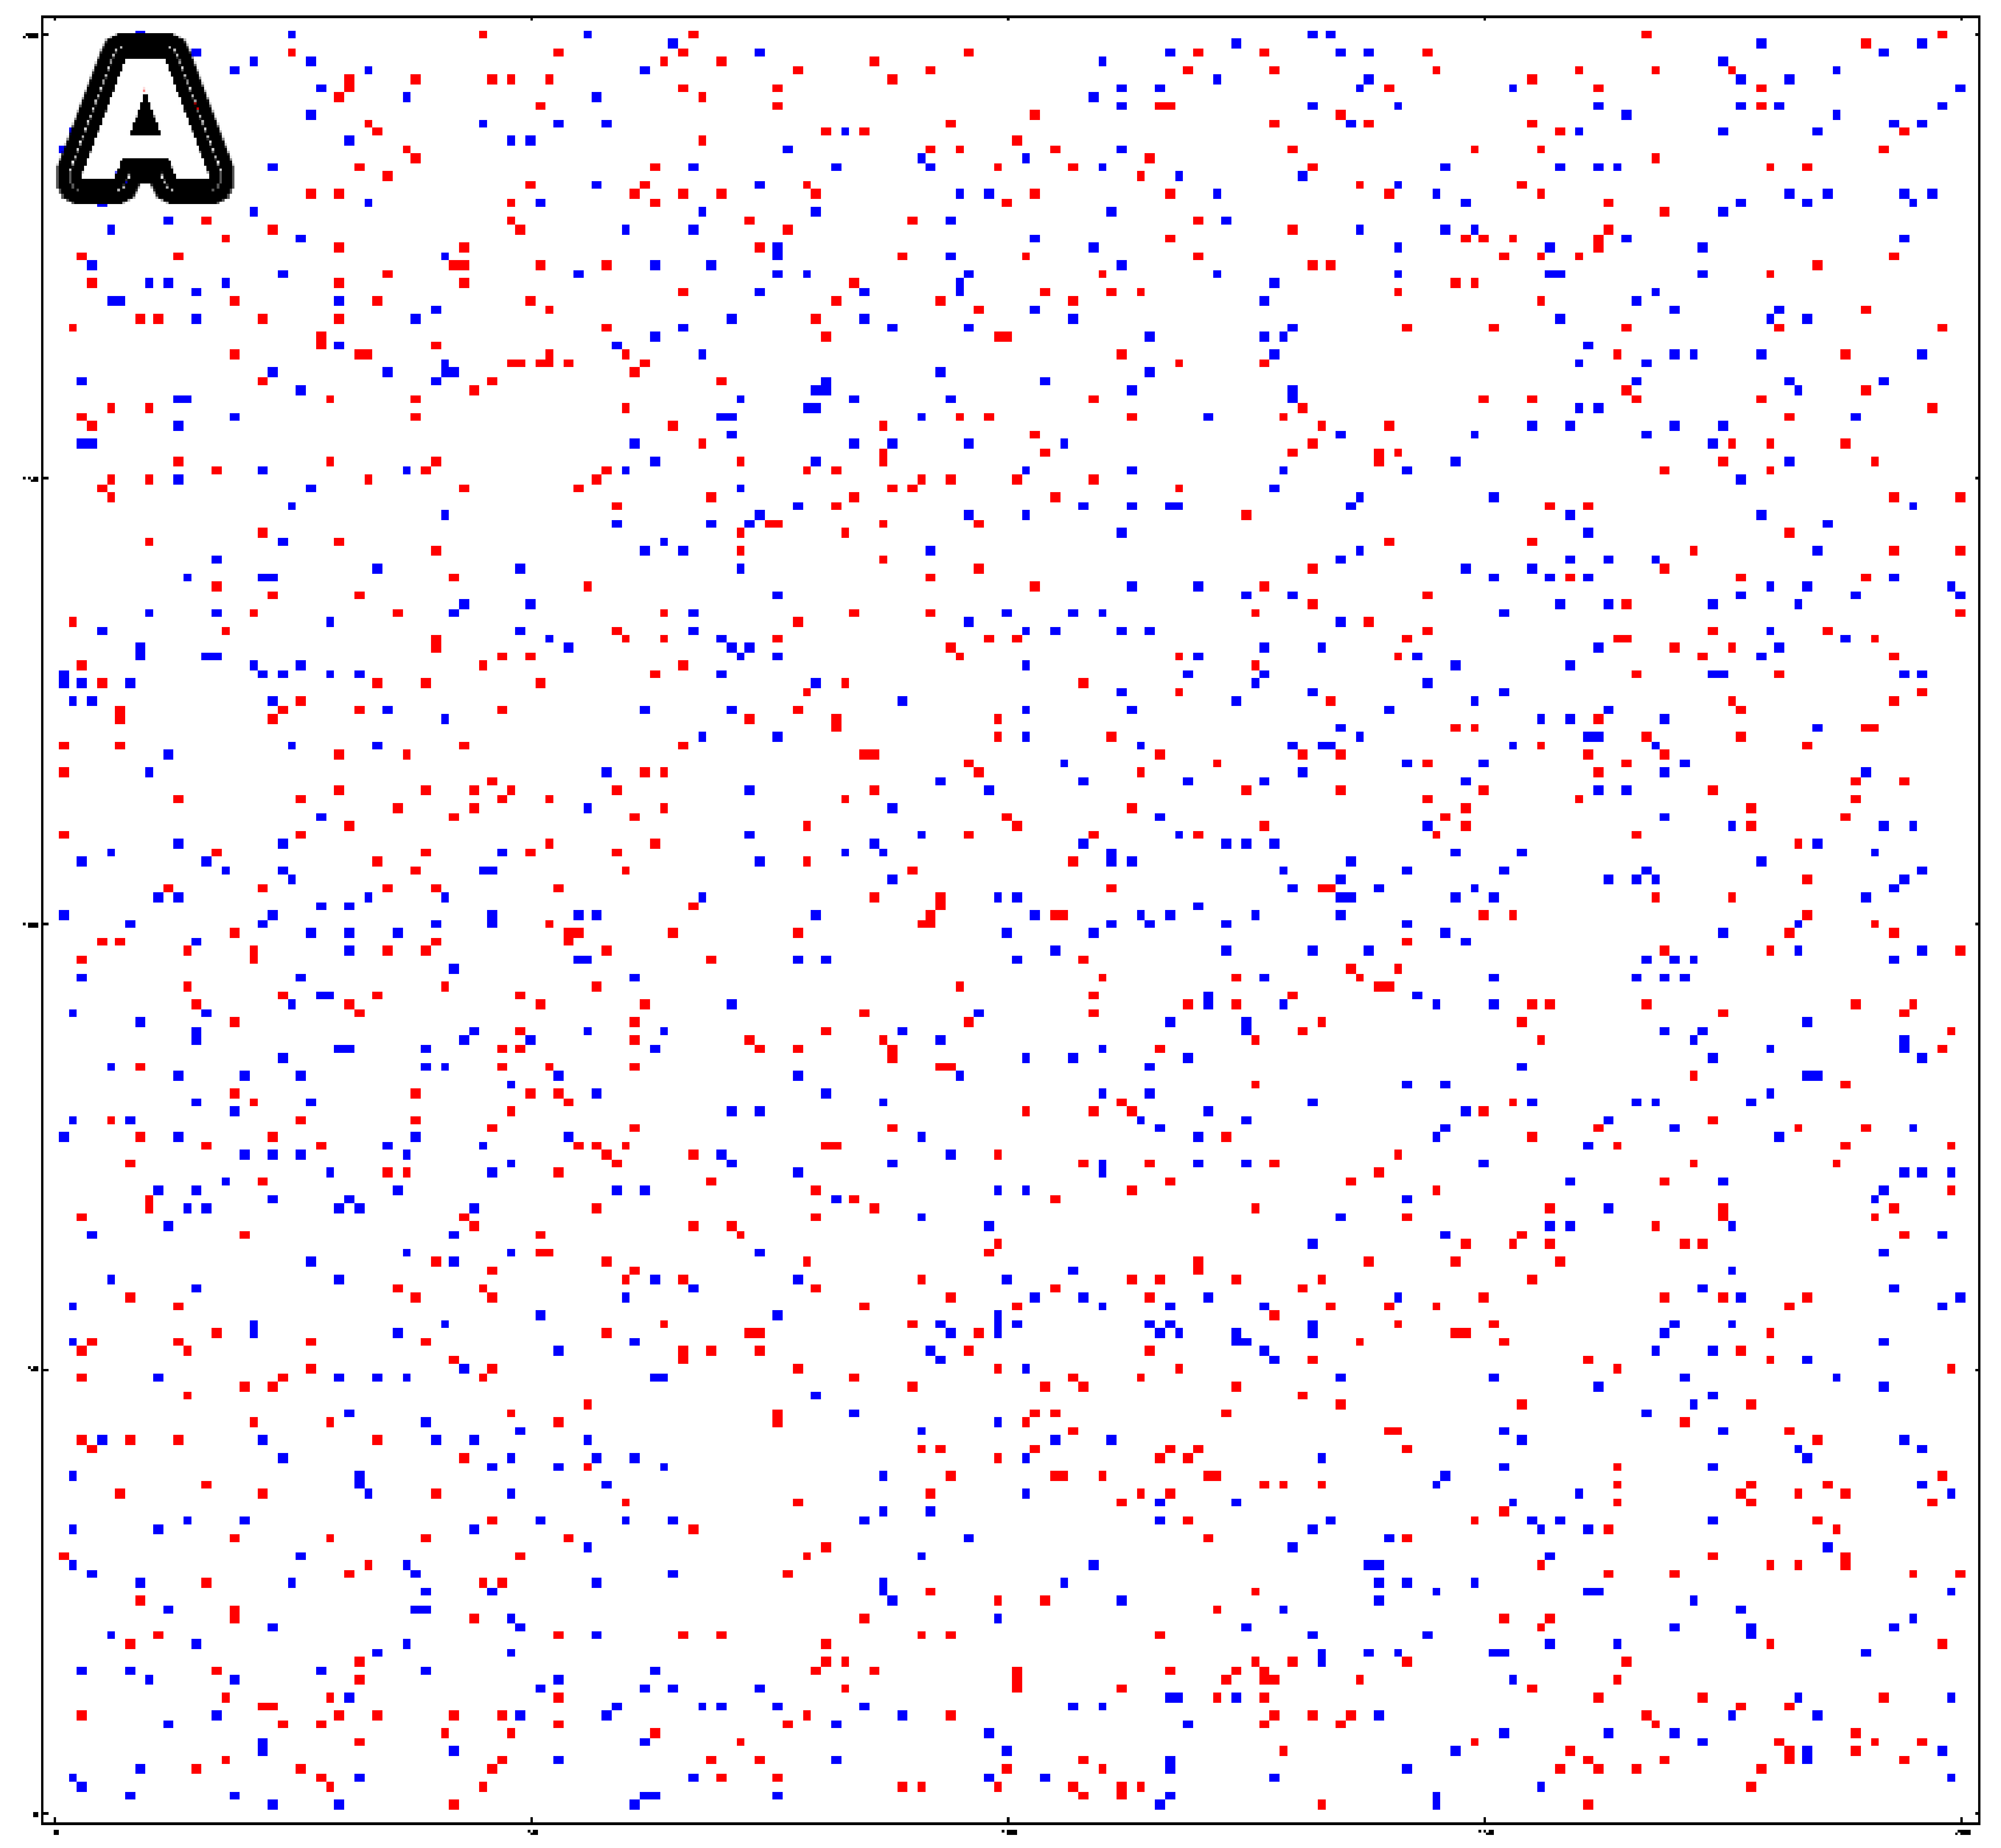
\includegraphics[width=0.25\textwidth]{imgs/02_010_heat1.eps}
%      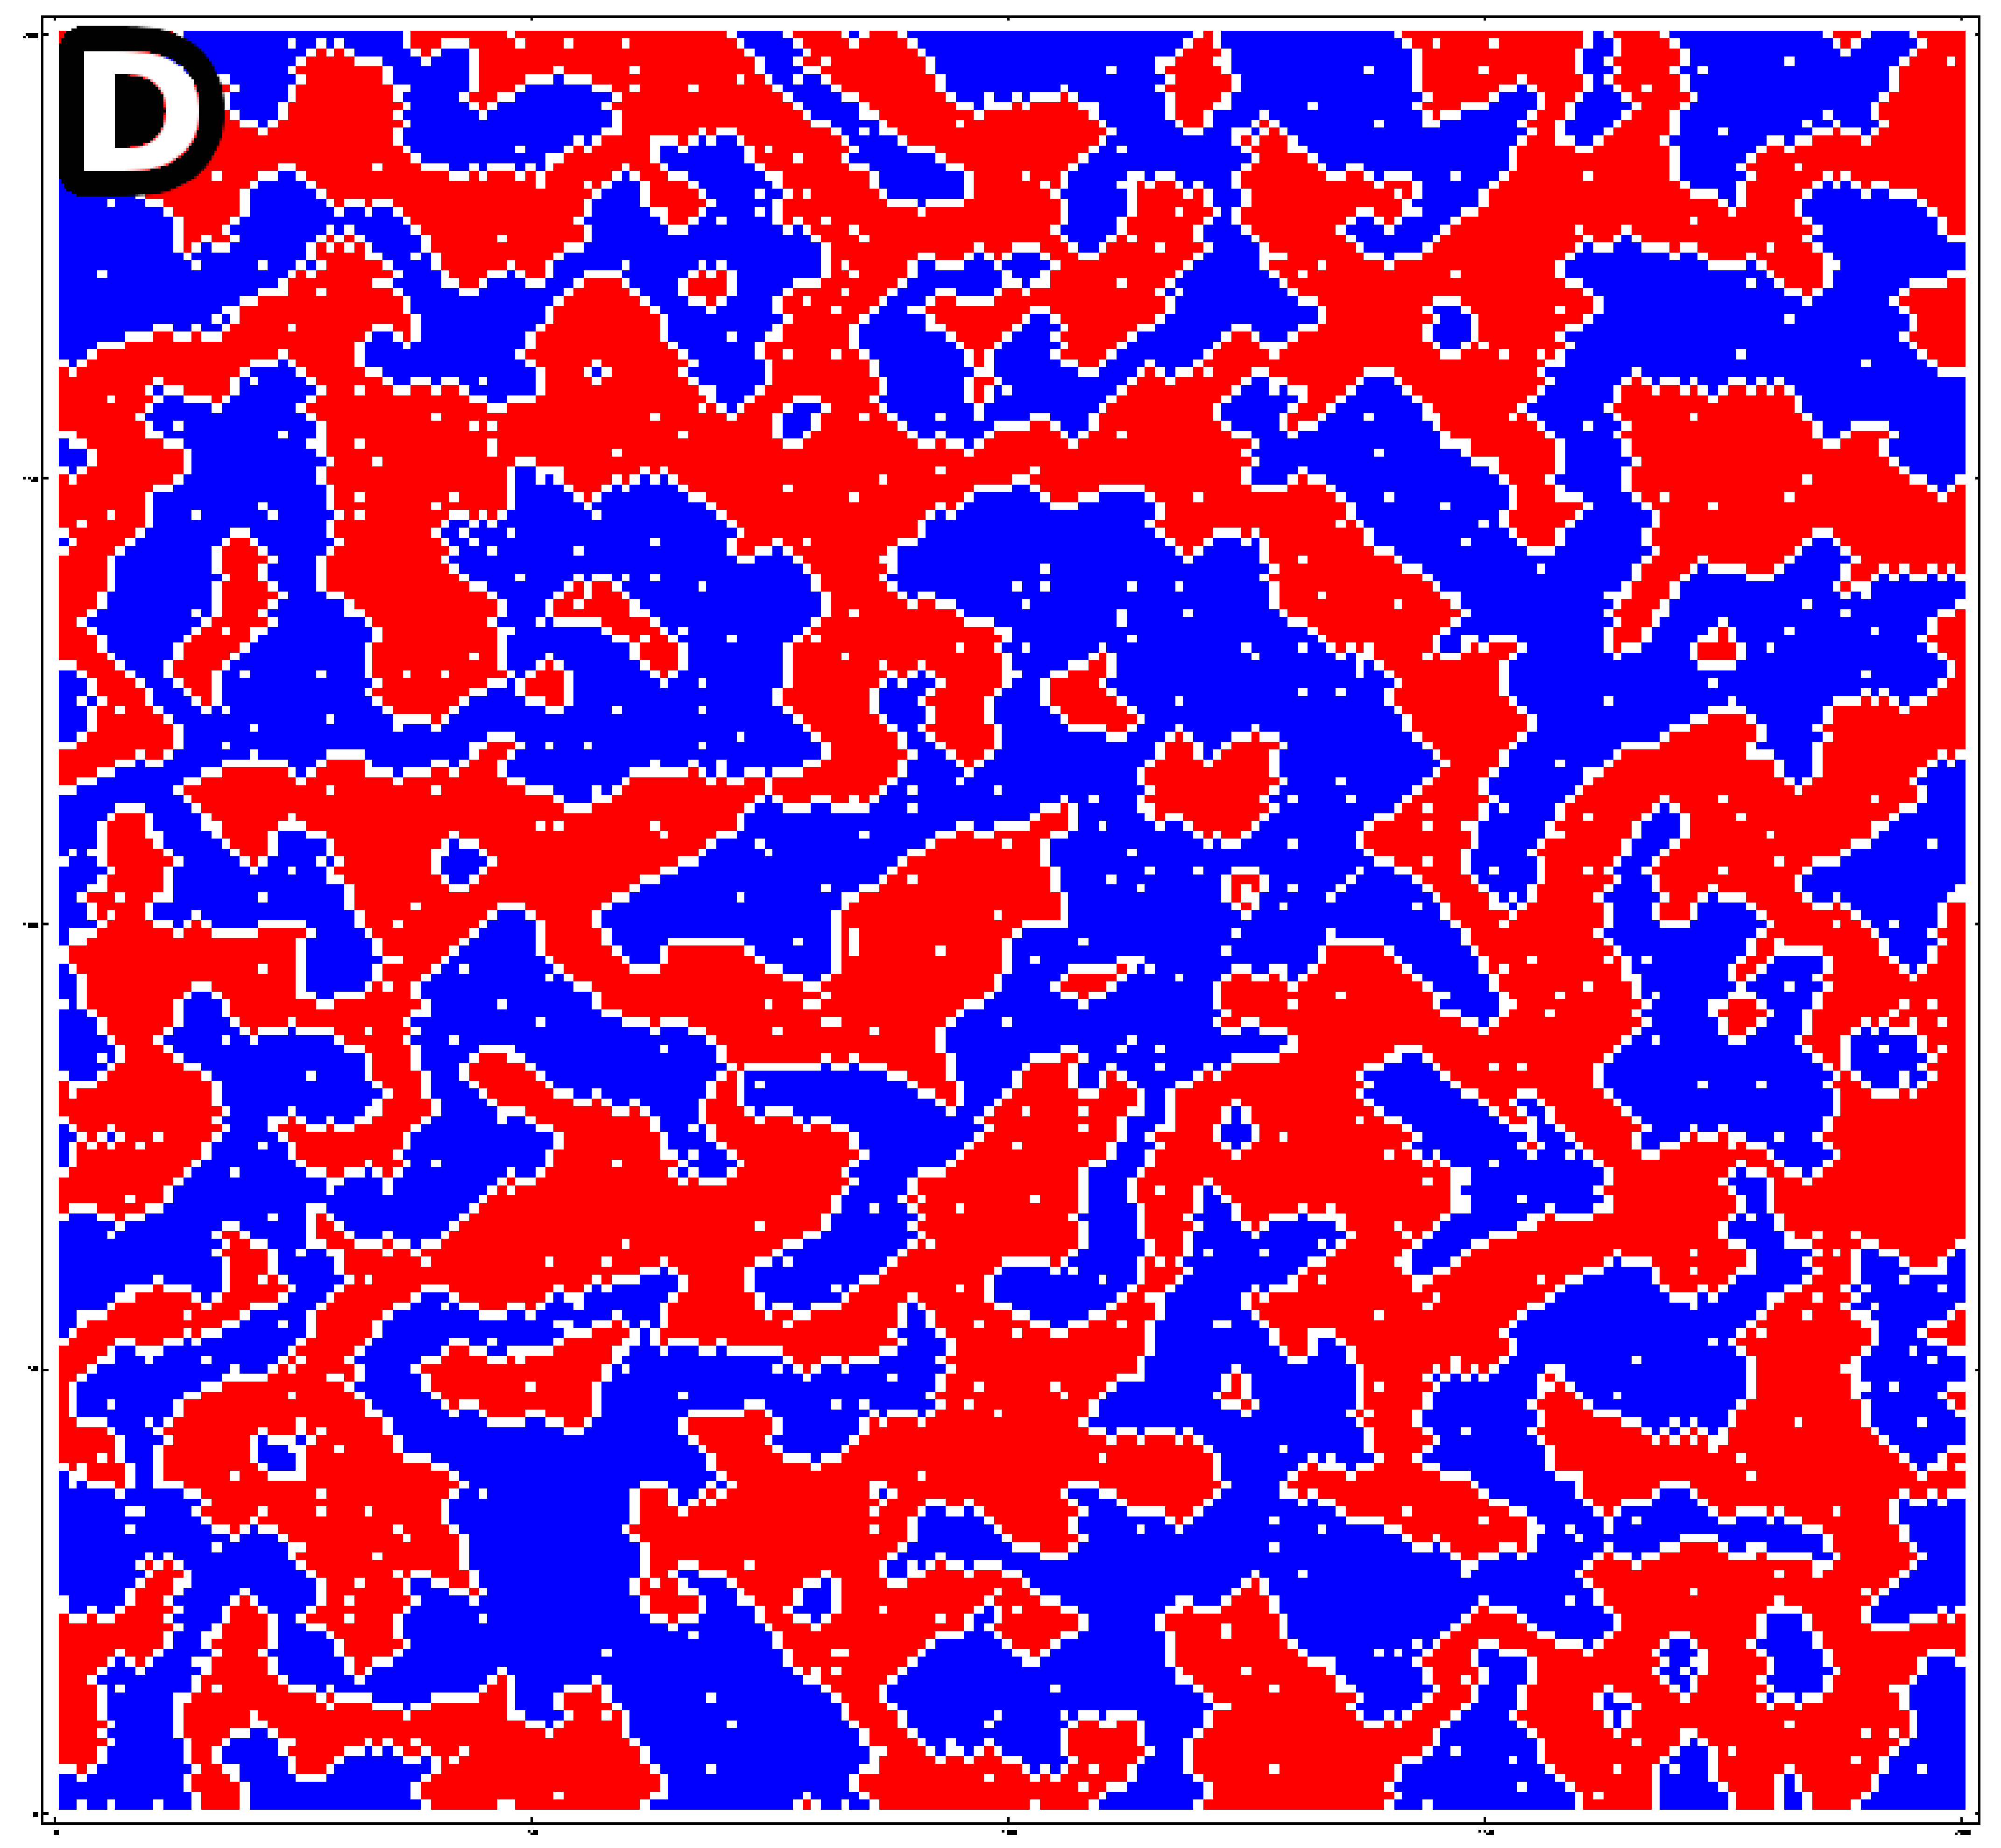
\includegraphics[width=0.25\textwidth]{imgs/02_010_heat64.eps}
%      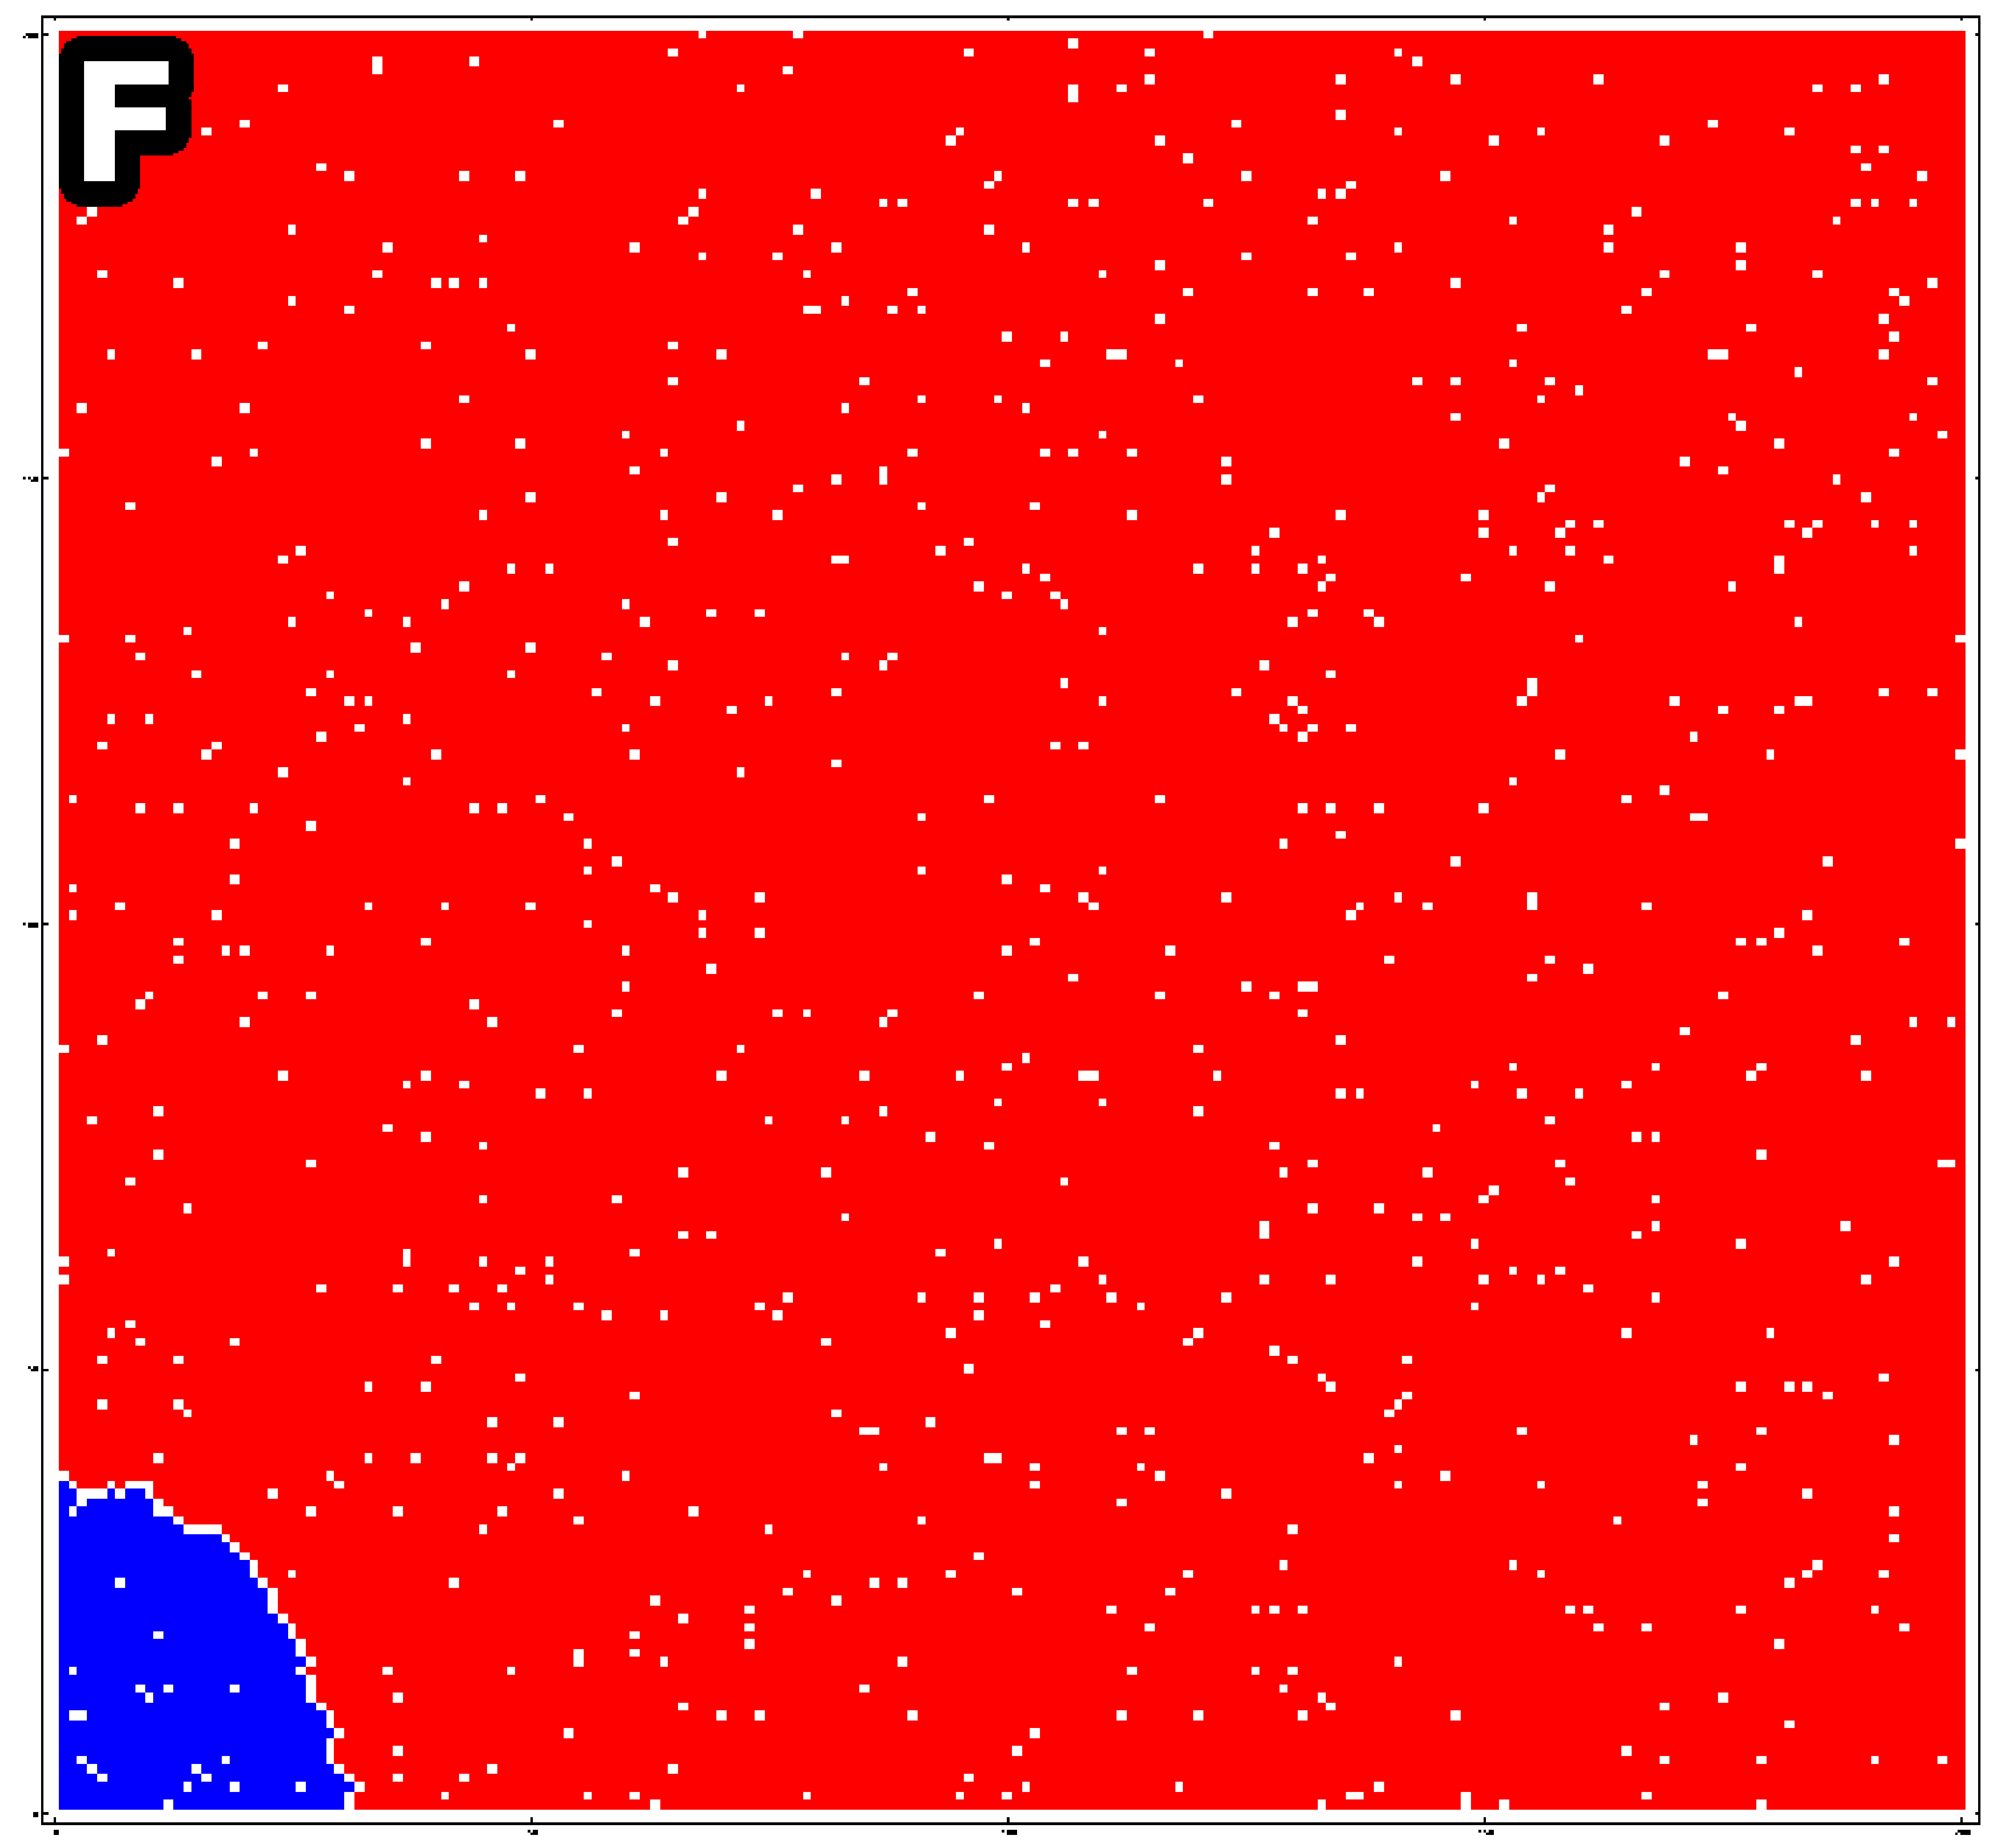
\includegraphics[width=0.25\textwidth]{imgs/02_010_heat93.eps}
%    \end{figure}
%
%    \column{0.55\textwidth}
%    \begin{itemize}
%    \item Dinâmica do padrão espacial. A população de células
%      tumorais cresce até prevalecer todo o domínio.
%      \vfill
%    \item Borda preenchida com células normais. Diâmetros de
%      exclusão se mostram determinantes para a prevalência do tipo
%      celular no estado estacionário.
%      \vfill
%    \item Aleatoriedade intrínseca. Na ausência de um fator que
%      diferencie os tipos celulares será a estocasticidade do
%      sistema que indicará qual tipo celular irá prevalecer.
%    \end{itemize}
%  \end{columns}
%\end{frame}
%
%\begin{frame}[plain,noframenumbering]{Agradecimentos}
%
%  \begin{columns}
%    \column{0.5\textwidth}
%    {\bf AMPhyBio}\\
%    Prof. Dr. Alexandre Ramos \\
%    Dr. Mauro Morais \\
%    Misaki Yamato \\
%    Suzy Lima \\
%    Leonardo Gama \\
%    André Gomes
%
%    \column{0.5\textwidth}
%    {\bf ICESP}\\
%    Profa. Dra. Fátima Pasini
%
%  \end{columns}
%
%  \vfill
%
%  \begin{figure}
%    \includegraphics[scale=0.25]{../imgs/icesp.png} \hfill
%    \includegraphics[scale=0.25]{../imgs/ffm.jpg} \hfill
%    \includegraphics[scale=0.5]{../imgs/capes.png}
%  \end{figure}
%\end{frame}

\begin{frame}[plain,noframenumbering]
  \titlepage
\end{frame}

\end{document}